%⠄⠄⠄⠄⠄⠄⣀⣀⣀⣤⣶⣿⣿⣶⣶⣶⣤⣄⣠⣴⣶⣿⣿⣿⣿⣶⣦⣄⠄⠄
%⠄⠄⣠⣴⣾⣿⠿⣿⣿⣿⣿⣿⣿⣿⣿⣿⣿⣿⣿⣿⣿⣿⣿⣿⣿⣿⣿⣿⣿⣦
%⢠⠾⣋⣭⣄⡀⠄⠄⠈⠙⠻⣿⣿⡿⠛⠋⠉⠉⠉⠙⠛⠿⣿⣿⣿⣿⣿⣿⣿⣿
%⡎⣾⡟⢻⣿⣷⠄⠄⠄⠄⠄⡼⣡⣾⣿⣿⣦⠄⠄⠄⠄⠄⠈⠛⢿⣿⣿⣿⣿⣿
%⡇⢿⣷⣾⣿⠟⠄⠄⠄⠄⢰⠁⣿⣇⣸⣿⣿⠄⠄⠄⠄⠄⠄⠄⣠⣼⣿⣿⣿⣿
%⢸⣦⣭⣭⣄⣤⣤⣤⣴⣶⣿⣧⡘⠻⠛⠛⠁⠄⠄⠄⠄⣀⣴⣿⣿⣿⣿⣿⣿⣿
%⠄⢉⣹⣿⣿⣿⣿⣿⣿⣿⣿⣿⣿⣷⣶⣦⣶⣶⣶⣶⣿⣿⣿⣿⣿⣿⣿⣿⣿⣿
%⢰⡿⠛⠛⠛⠛⠻⠿⠿⢿⣿⣿⣿⣿⣿⣿⣿⣿⣿⣿⣿⣿⣿⣿⣿⣿⣿⣿⣿⣿
%⠸⡇⠄⠄⢀⣀⣀⠄⠄⠄⠄⠄⠉⠉⠛⠛⠻⠿⣿⣿⣿⣿⣿⣿⣿⣿⣿⣿⣿⣿
%⠄⠈⣆⠄⠄⢿⣿⣿⣿⣷⣶⣶⣤⣤⣀⣀⡀⠄⠄⠉⢻⣿⣿⣿⣿⣿⣿⣿⣿⣿
%⠄⠄⣿⡀⠄⠸⣿⣿⣿⣿⣿⣿⣿⣿⣿⣿⣿⣿⠂⠄⢠⣿⣿⣿⣿⣿⣿⣿⣿⣿
%⠄⠄⣿⡇⠄⠄⣿⣿⣿⣿⣿⣿⣿⣿⣿⣿⡿⠃⠄⢀⣼⣿⣿⣿⣿⣿⣿⣿⣿⣿
%⠄⠄⣿⡇⠄⠠⣿⣿⣿⣿⣿⣿⣿⣿⡿⠋⠄⠄⣠⣾⣿⣿⣿⣿⣿⣿⣿⣿⣿⣿
%⠄⠄⣿⠁⠄⠐⠛⠛⠛⠛⠉⠉⠉⠉⠄⠄⣠⣾⣿⣿⣿⣿⣿⣿⣿⣿⣿⣿⣿⡿
%⠄⠄⠻⣦⣀⣀⣀⣀⣀⣀⣤⣤⣤⣤⣶⣾⣿⣿⣿⣿⣿⣿⣿⣿⣿⣿⣿⡿⠋⠄

\documentclass{article}
\title{Electromagnetic Compatibility}
\date{2021}
\author{Jacopo Ferretti}
\usepackage[utf8]{inputenc} % Required for inputting international characters

\newcommand\vertarrowbox[3][3ex]{%
  \begin{array}[t]{@{}c@{}} #2 \\
  \left\uparrow\vcenter{\hrule height #1}\right.\kern-\nulldelimiterspace\\
  \makebox[0pt]{\scriptsize#3}
  \end{array}%
}
\usepackage[nottoc]{tocbibind}
\usepackage{amsmath,amssymb,bm,mathtools}
\usepackage{pgfplots}
\pgfplotsset{compat=1.13}
\usepgfplotslibrary{smithchart}
\usepgfplotslibrary{polar}
\usepackage{steinmetz}
\usepackage[makeroom]{cancel}
\numberwithin{equation}{section}
\numberwithin{figure}{section}
\newcommand{\ihat}{\hat{\imath}}
\newcommand{\jhat}{\hat{\jmath}}
\newcommand{\khat}{\hat{\mathnormal{k}}}
\newcommand{\phas}[1]{\overset{\mathbin
{{\circ \mkern-2.5mu\rightarrow}}}{#1}}
\usepackage[a-2b]{pdfx}
\usepackage[pdfa]{hyperref}
\usepackage{cleveref}
\usepackage{pgfplots}
\usepackage{xcolor}
\usepackage{circuitikz}
\usetikzlibrary{positioning} 
\usepackage{float}
\usepackage{scalerel}
\usepackage{siunitx}
\newcommand{\bottomPlus}{\ensuremath{_{\scaleto{+}{3pt}}}}
\newcommand{\bottomMinus}{\ensuremath{_{\scaleto{-}{3pt}}}}
\sisetup{
  per-mode=fraction,
  fraction-function=\tfrac
}
\pgfplotsset{compat=1.17}

%% stupid dunno emoticon%%
\newcommand{\dunno}[1][]{%
\begin{tikzpicture}[baseline,x=0.8\ht\strutbox,y=0.8\ht\strutbox,line width=0.125ex,#1]
\def\arm{(-2.5,0.95) to (-2,0.95) (-1.9,1) to (-1.5,0) (-1.35,0) to (-0.8,0)};
\draw \arm;
\draw[xscale=-1] \arm;
\def\headpart{(0.6,0) arc[start angle=-40, end angle=40,x radius=0.6,y radius=0.8]};
\draw \headpart;
\draw[xscale=-1] \headpart;
\def\eye{(-0.075,0.15) .. controls (0.02,0) .. (0.075,-0.15)};
\draw[shift={(-0.3,0.8)}] \eye;
\draw[shift={(0,0.85)}] \eye;
% draw mouth
\draw (-0.1,0.2) to [out=15,in=-100] (0.4,0.95); 
\end{tikzpicture}}
%-----------------------%
\usepackage{steinmetz}
\usepackage{pifont}% http://ctan.org/pkg/pifont

\begin{document}
\maketitle
\begin{center}
  \vspace*{\stretch{0.5}}
  \Huge{\ding{166}}
  \vspace*{\stretch{1.5}}
\end{center}
\newpage
\tableofcontents
\newpage
\section*{Introduction}
\addcontentsline{toc}{section}{Introduction}
I share with you my work, it is not perfect, but i think it could be helpful for anyone.\\
You can share it, modify or do whatever you want, i enjoy to write in \LaTeX, so i'm totally fine with this.\\
Please consider to help me to find any mistakes or misunderstanding, contact me or just modify the code from Github.\\
If you want to be added to my private Github repository just give me your email and I'll add you with no problem.\\
I want to suggest you to give a look at the book \emph{High Speed Digital Design}\cite{zhang_book}, in the introduction it is explained in very simple and intuitive way the first part of our course.\\
\begin{footnotesize}
  You can find it easily in 1lib.eu but i didn't told you nothing :x
\end{footnotesize}
\newpage
\section{Class 1 - 22/02/21}
Today's lesson was a recap on Maxwell equation.\\
First of all we have seen the Faraday equation:
\begin{equation}\label{eq:first_maxwell}
 \oint_l \overline{E} \cdot \hat{l} \, dl = -\frac{d}{dt}\int_s \overline{B} \cdot \hat{n} \, ds = - \frac{d\Phi_B}{dt}
\end{equation}
And this second equation:
\begin{equation}
\oint_l \overline{H}\cdot \hat{l} \, dl = \int_s \left(\frac{d\overline{D}}{dt}+\overline{J}\right)\cdot \hat{n}\,ds
\end{equation}
Where those symbol are:
\begin{itemize}
\item $E=$ intensity of electric field $[\frac{V}{m}]$
\item $B=$ magnetic induction vector $[T]$
\item $H=$ intensity magnetic field $[A]$
\item $D=$ electronic displacement $[\frac{A}{m}]$
\item $J=$ intensity of electric current $[\frac{A}{m^2}]$
\end{itemize}
Now, we can think $E - H$ as the element measuring the real electromagnetic field, and $D - B$ as something that measure the effect of the EMF.\\
We also remember that:
\begin{equation}\label{eq:1}
\frac{d}{dt}\int_V \overline{\rho} \, dV=-\int_s \overline{J}\cdot \hat{n}\,ds
\end{equation}
Where $\rho$ is the density of charge (volumetric) and $s$ is the boundary of the volume $V$ in the integral on the left.\\
On the right of \cref{eq:1} we can find a minus sign, because if my electron goes from out to in in our volume, it means that the current is going from in to out (the right integral is positive because of the conversion for the versor $\hat{n}$ that goes from in to out). If the the electron are going in as we already said, we are accumulating a negative charge, for this reason we need to put this negative sign.
\subsection*{Recap of operator nabla}
\subsubsection*{Gradient $\nabla T$}
Usually we refer to a variation of a scalar quantity with the derivative (for example $\frac{dT}{dt}$).\\
If the scalar $T$ variates in more than one component, we want have a look at the derivative of everything: $\frac{dT}{dx},\frac{dT}{dy},\frac{dT}{dz}$.\\
If we are in space, our scalar field vary his value over we have 3 components, so we introduce the \emph{gradient} of the scalar field T (temperature) as:
\begin{equation}
\left(\frac{\partial T}{\partial x}\ihat+\frac{\partial T}{\partial y}\jhat+\frac{\partial T}{\partial z}\khat\right)=\nabla\,T
\end{equation}
Where $\nabla=\frac{\partial}{\partial x}\ihat +\frac{\partial}{\partial y}\jhat +\frac{\partial}{\partial z}\khat$ is the nabla operator.\\
Now from the scalar $T$ we obtained a vector and that is okay, but if our field is not scalar but vectorial?\\
The electric field $\overline{E}=E_x \ihat + E_y \jhat + E_z \khat$ is a vectorial field.
What we can do now is using the dot or cross product between our vector E and the $\nabla$ operator.
\subsubsection*{Scalar product (divergence) $\nabla \cdot \overline{E}$}
The scalar product (dot) between nabla and a vectorial field is named \emph{divergence}
\begin{equation}
\nabla \cdot \overline{E} =\frac{\partial E_x}{\partial y}+\frac{\partial E_y}{\partial y}+\frac{\partial E_z}{\partial z}
\end{equation}
Physically speaking the divergence of the vector $E$ is \textit{how $E_x$ is changing over the $x$ direction etc...}\\
Another way to look at this divergence is:
\begin{equation}
\nabla \cdot \overline{E} = \cdots = \lim_{\Delta v \rightarrow 0}\frac{\oint_s \overline{E}\cdot \hat{n}\, ds}{\Delta v}
\end{equation}
\subsubsection*{Divergence theorem}
This theorem is very useful to transform an integral over a surface to an integral over a volume.
\begin{equation}
\int_v \nabla \cdot \overline{E} = \int_s \overline{E}\cdot \hat{n}\,ds
\end{equation}
So the integral of the divergence over a volume is equal to the flux across the boundary surface of the volume.
\subsubsection*{Cross product (curl) $\nabla \times \overline{E}$}
The cross product of nabla and our vectorial field is named \emph{curl}
\begin{align}
    \begin{split}
        \nabla\times \overline{E}&=det
        \left[ \begin{matrix}
        \ihat & \jhat & \khat\\
        \frac{\partial}{\partial x} & \frac{\partial}{\partial y} & \frac{\partial}{\partial z}\\
        E_x & E_y & E_z
        \end{matrix}\right]=\\[5pt]
        &=\left(\frac{\partial E_x}{\partial y} - \frac{\partial E_y}{\partial z}\right)\ihat+
        \left(\frac{\partial E_x}{\partial z} - \frac{\partial E_z}{\partial x}\right)\jhat+
        \left(\frac{\partial E_y}{\partial x} - \frac{\partial E_x}{\partial y}\right)\khat
    \end{split}
\end{align}
The curl (as the name in italian \emph{rotore} says) explains the behavior of $E_x$ (for example).\\
Again, another way to look at the curl is:
\begin{equation}
\nabla \times \overline{E}=\lim_{\Delta s \rightarrow 0}\frac{\hat{n}\cdot\oint_l \overline{E}\cdot \hat{l}\,dl}{\delta s}
\end{equation}
The $\hat{n}$ is there to maximize the value of $\oint_l \overline{E}\cdot \hat{l}\,dl$. I don
't really know why, PLEASE GIVE IT A LOOK.\\
Note that we are not using the vector symbol over the nabla because we are not multiplying two vector, instead nabla is an \emph{operator} as $\cdot$, $\sin$ or$\oplus$, so we don't write $\xcancel{\overline{\nabla}\cdot\overline{E}}$
\subsection*{Stokes Theorem}
This theorem is similar to divergence theorem, but instead of surface and volume, we deal with surface and line:
\begin{equation}\label{eq:stokes_eq}
\int_s \nabla\times \overline{E}\cdot \hat{n}\,ds=\oint_l\overline{E}\cdot\hat{l}\,dl
\end{equation}
It means that the flux over a surface of the curl of a vectorial field, is the integral of that field on the line that is bounding s.
\subsubsection*{Laplacian}\label{sec:laplacian}
If i use the operator curl twice we get the laplacian.\\
Consider the gradient of a scalar field $T$: $\nabla T=\left(\frac{\partial T}{\partial x}\ihat+\frac{\partial T}{\partial y}\jhat+\frac{\partial T}{\partial z}\khat\right)$ now:
\begin{equation}\label{eq:2}
\nabla\cdot(\nabla T)=\nabla^2T=\left(\frac{\partial^2 T}{\partial x^2}+\frac{\partial^2 T}{\partial y^2}+\frac{\partial^2 T}{\partial z^2}\right)
\end{equation}
If we consider a vectorial field $\overline{E}=E_x \ihat + E_y \jhat + E_z \khat$
\begin{equation}
\nabla^2\cdot \overline{E}= \nabla^2E_x\,\ihat+\nabla^2E_y\,\jhat+\nabla^2E_z\,\khat
\end{equation}
Actually we can write $\nabla^2E_x\,\ihat+\nabla^2E_y\,\jhat+\nabla^2E_z\,\khat$ because we are dealing with different Laplacian for each $E$ component, that is scalar.\\
The same can be said to $\nabla^2 T$ on \cref{eq:2}
\subsubsection*{Going back to the Stokes Theorem}
With stokes theorem we can write something similar to the first Maxwell equation:\\
Starting from the first Maxwell equation seen in \cref{eq:first_maxwell}
\begin{equation}
\oint_l \overline{E} \cdot \hat{l} \, dl = -\frac{d}{dt}\int_s \overline{B} \cdot \hat{n} \, ds
\end{equation} 
And with the Stokes theorem \cref{eq:stokes_eq}, we can write:
\begin{equation}
\int_s (\nabla \times \overline{E})\cdot \hat{n}\,ds=\frac{d}{dt}\int_s \overline{B}\cdot\hat{n}\, ds
\end{equation}
We notice that we have two integral over the same surface $s$, so:
\begin{equation}
\int_s \left(\nabla\times\overline{E}+\frac{d\overline{B}}{dt}\right)\cdot\hat{n}\,ds=0
\end{equation}
Finally we know that this integral is equal to zero if the equation inside the brackets is also equal to zero, so:
\begin{equation}\label{eq:maxwell_first_local}
\nabla\times\overline{E}=-\frac{d\overline{B}}{dt}
\end{equation}
This \cref{eq:maxwell_first_local} can be considered as the first Maxwell equation but for a point.\\
We can do the same for the second Maxwell equation:
\begin{equation}\label{eq:maxwell_second_local}
\nabla\times\overline{H}=\frac{d\overline{D}}{dt}+\overline{J}
\end{equation}
\cref{eq:maxwell_first_local} and \cref{eq:maxwell_second_local}are also named as the local formulation of the Maxwell equation.\\
To be more precise we can actually split the intensity of current $J$ in two contribution:
\begin{itemize}
\item $J_\sigma$: current generated by the electromagnetic field on iron ($\sigma$ actually is the conductivity).
\item $J_i$: current that generates the electromagnetic field, given by for example a battery of the phone.
\end{itemize}
We have seen $J_\sigma$ as the metallic behavior of the receiver and $J_i$ as the source of the EMF, and we can also see at the component $\frac{d\overline{D}}{dt}$ as he behavior of the dielectric material due to the displacement of the charge.\\
\cref{eq:maxwell_second_local} becomes:
\begin{equation}
\nabla\times\overline{H}=\frac{d\overline{D}}{dt}+\overline{J}_\sigma+\overline{J}_i
\end{equation}
\subsection*{Step forward: solution of the Maxwell equation}
The solutions of the Maxwell equations are not always simple to obtain analytically, we need to have a sort of classification for the equation to be solved. Those can be classified as:
\begin{itemize}
\item \textbf{Linear} and \textbf{non linear}
\item \textbf{isotropic} and \textbf{anisotropic}
\item \textbf{stationary} and \textbf{non stationary}
\item \textbf{dispersive} and \textbf{non dispersive}
\begin{itemize}
\item in time
\item in space
\end{itemize}
\end{itemize}
\textbf{Linear} means that the equation is composed only and only only by the sum of each variable $x_i$ multiplied by their own coefficient $a_i$: $\bm{a_1x_2+a_1x_2\cdots + a_nx_n+b=0}$, this is an important class of equation because we can use a lot of useful properties.\\
\textbf{Stationary} means that the results will not change with the time, so if i do the experiment now or 10 years later I'll be sure that nothing will change.\\
We need this little recap to neglect all those non optimal behavior, and for the sake of simplicity we use those relation:
\begin{itemize}
    \item $\overline{D}=\varepsilon \overline{E}\;\rightarrow \varepsilon$ is the dielectric permittivity
    \item $\overline{B}=\mu \overline{H}\;\rightarrow \mu$ is the electric permeability
    \item $\overline{J_\sigma}=\sigma \overline{E}\;\rightarrow \sigma$ is the conductivity (is there when we have a metallic object)
\end{itemize}
Those are very oversimplified, but can be useful to study our EMF.\\
We remember that we have obtained the $\varepsilon \, \mu \, \sigma$ value in vacuum, that are:
\begin{itemize}
    \item $\varepsilon_0=\frac{1}{36\pi}\,10^{-9} \left[\frac{F}{m}\right]$
    \item $\mu_0=4\pi\,10^{-7} \left[\frac{H}{m}\right]$
    \item $\sigma_0=0 \left[\frac{S}{m}\right]$
\end{itemize}
When we are dealing with linear material, we can not consider the numeric value of these constant over vacuum, but instead with some approximation we can consider:
\begin{itemize}
    \item $\varepsilon=\varepsilon_0\,\varepsilon_r$
    \item $\mu=\mu_0\,\mu_r$
    \item $\sigma=\frac{1}{\rho}$
\end{itemize}
Now, the first two local Maxwell equation which we have already seen are:
\begin{equation}\label{eq:maxwell_system_2}
    \begin{cases}
    \nabla\times\overline{E}=-\frac{d\overline{B}}{dt}\\[5pt]
    \nabla\times\overline{H}=\frac{d\overline{D}}{dt}+\overline{J}_\sigma +\overline{J}_i
    \end{cases}
\end{equation}
We try to make this system solvable by substitution:
\begin{equation}\label{eq:maxwell_system}
    \begin{cases}
    \nabla\times\overline{E}=-\mu\frac{d\overline{H}}{dt}\\[5pt]
    \nabla\times\overline{H}=\varepsilon\frac{d\overline{E}}{dt}+\sigma\,\overline{E}+\overline{J}_i
    \end{cases}
\end{equation}
As can be seen, the system in \cref{eq:maxwell_system} is a systems of equations in two unknown variable ($E$ and $H$), we can solve that but it would be very complicated.
\subsection*{Another useful equation}
similarly to what we have done in \cref{eq:maxwell_first_local}, we can write this equation exploiting the Stokes Theorem (\cref{eq:stokes_eq}):
    \begin{align}
    \begin{split}
    &\frac{d}{dt}\int_v\overline{\rho}\,dv=-\int_s \overline{J}\cdot \hat{n}ds=-\int_v\nabla\cdot\overline{J}\,dv\\[5pt]
    &\int_v\left(\frac{d\overline{\rho}}{dt}+\nabla\cdot\overline{J}\right)\,dv=0
    \end{split}
    \end{align}
Then we obtain:
\begin{equation}
    \nabla\cdot\overline{J}=-\frac{d\overline{\rho}}{dt}
\end{equation}
\subsection*{Third maxwell equation in local formulation}
First of all we try to do the divergence of $\nabla\times\overline{E}$.\\ 
Note that the result of the divergence of a curl is equal to zero because the result of the curl will be perpendicular to the nabla operator, so $\nabla\cdot(\nabla\times\overline{E})=0$
\begin{align}
    \begin{split}
        &\nabla \cdot \left[ (\nabla\times \overline{E})=-\frac{d\overline{B}}{dt}\right]=\\[5pt]
        &\nabla \cdot \left(-\frac{d\overline{B}}{dt}\right)=0\\[5pt]
        &\frac{d}{dt}(\nabla\cdot \overline{B})=0
    \end{split}
\end{align}
We obtained the \emph{Third maxwell equation in local formulation}:
\begin{equation}\label{eq:third_max_eq_local}
    \nabla\cdot \overline{B}=0
\end{equation}
We can say that \cref{eq:third_max_eq_local} ist true because we are considering that at the starting time $t_0$ our EMF was turned off ($\nabla\cdot \overline{B}=0 $ at $t_0$).
If $\mu$ is constant:
\begin{equation}
    \nabla\cdot \overline{B}=\nabla\cdot(\mu\,\overline{H})=\nabla\cdot\overline{H}=0
\end{equation}
\subsection*{Forth maxwell equation in local formulation}
Using the same passages as before, we can obtain the forth maxwell equation in local formulation by doing the divergence of the curl of $H$
\begin{align}
    \begin{split}
        &\nabla \cdot \left[ (\nabla\times \overline{H})=-\frac{d\overline{D}}{dt}+\overline{J}\right]=\\[5pt]
        &\nabla \cdot \left(-\frac{d\overline{D}}{dt}+\overline{J}\right)=0\\[5pt]
        &\frac{d}{dt}(\nabla\cdot \overline{D})+\nabla\cdot \overline{J}=0\\[5pt]
        &\frac{d}{dt}(\nabla\cdot \overline{D})+\nabla\cdot \frac{d\overline\rho}{dt}=0\\[5pt]
        &\frac{d}{dt}\left(\nabla\cdot\overline{D}-\overline{\rho}\right)=0\\[5pt]
    \end{split}
\end{align}
At the end, the Forth maxwell equation in local formulation is:
\begin{equation}
    \nabla\cdot\overline{D}=\overline{\rho}
\end{equation}
If $\varepsilon$ is constant we obtain
\begin{align}
    \begin{split}
        &\nabla\cdot(\varepsilon\,\overline{E})=\overline{\rho}\\[5pt]
        &\nabla\cdot\overline{E}=\frac{\overline{\rho}}{\epsilon}
    \end{split}
\end{align}
Those equation does not say anything more than the maxwell equation.
To summarize all the equation we have obtained (for some reason):
\begin{center}
\begin{tabular}{ c c }
    $\nabla\cdot\overline{E}=\frac{\overline{\rho}}{\epsilon}$&$\nabla\cdot\overline{J}=-\frac{d\overline{\rho}}{dt}$\\[5pt]
    $\nabla\cdot\overline{B}=0$&$\nabla\cdot\overline{D}=\rho$
\end{tabular}
\end{center}
\section{Class 2 - 26/02/21}
\subsection*{Vector wave equation}
Here we go again, today from \cref{eq:maxwell_system} we want to obtain the wave equation of the EMF, we will make a lot of simplification.\\
First of all we consider:
\begin{itemize}
    \item No accumulated charge (source free, no current that generates the EMF) $\boldsymbol{\overline{J_i}=0}$
    \item No losses (nonconducting medium) $\boldsymbol{\overline{J_i}$ $\sigma \cdot\overline{E}}$
\end{itemize}
Then from \cref{eq:maxwell_system} we now have:
\begin{equation}\label{eq:maxwell_simplified}
    \begin{cases}
    \nabla\times\overline{E}=-\mu\frac{\partial \overline{H}}{\partial t}\\[5pt]
    \nabla\times\overline{H}=\varepsilon\frac{\partial \overline{E}}{\partial t}
    \end{cases}
\end{equation}
We continue to try to find the wave equation by using some tricks, the next passage is to apply the curl on the first equation from \cref{eq:maxwell_simplified}.
\begin{align}
    \begin{split}
        \nabla\times\nabla\times\overline{E}=&-\nabla\times\mu \frac{\partial \overline{H}}{\partial t}=-\mu \frac{\partial}{\partial t} \nabla\times \overline{H}\\[5pt]
        &=-\mu \frac{\partial}{\partial t}\varepsilon\frac{\partial \overline{E}}{\partial t}=\\[5pt]
        &=-\mu \varepsilon \frac{\partial^2\overline{E}}{\partial t^2}
    \end{split}
\end{align}
We remember a cool property of the curl of a curl of a vector field:
\begin{equation}
    \nabla\times\nabla\times\overline{E}=\nabla(\nabla\cdot \overline{E})-\nabla^2\,\overline{E}
\end{equation}
Please note that we have already discussed the $\nabla^2$ symbol before in \cref{sec:laplacian} as the Laplacian. Now let's write:
\begin{equation}
    \nabla(\nabla\cdot \overline{E})-\nabla^2\,\overline{E}=-\mu \varepsilon \frac{\partial^2\overline{E}}{\partial t^2}
\end{equation}
We simplify a little bit more, and we consider that we don't have free charge: $\nabla(\varepsilon \overline{E}=0)$ and we obtain:
\begin{equation}\label{eq:whave_1}
    \nabla^2\,\overline{E}-\mu \varepsilon \frac{\partial^2\overline{E}}{\partial t^2}=0
\end{equation}
WE FINALLY OBTAINED THE \emph{WAVE EQUATION}. Here we define a constant that will be helpful next:
\begin{equation}
    c=\frac{1}{\sqrt{\mu\varepsilon}}
\end{equation}
Then \cref{eq:whave_1} becomes:
\begin{equation}\label{eq:whave_2}
    \nabla^2\,\overline{E}-\frac{1}{c^2} \frac{\partial^2\overline{E}}{\partial t^2}=0
\end{equation}
Pay attention to one thing: if you look at the maxwell equation \cref{eq:maxwell_simplified} it is a differential equation of the first order, but now we have a second order differential equation (\cref{eq:whave_2}) and the set of solution is increased. We don't address this problem now, but keep in mind that later we will be able to select the good solution by using the divergence equation (\textsl{i don't really know what does it mean}).\\
If instead use the second equation from \cref{eq:whave_2}, and we do all the passages as before, we obtain nearly the same equation, but with $\overline{H}$
\begin{equation}
    \nabla^2\,\overline{H}-\frac{1}{c^2} \frac{\partial^2\overline{H}}{\partial t^2}=0
\end{equation}
\subsection*{Scalar wave equation}
Now let's try to write our equation with scalars and not vectors, it should simplify a bit.\\
If we consider the vector $E$ to be completely parallel to the $z$ axes, it means:
\begin{equation}
    \overline{E}(x,y,z)=\xcancel{E_x\ihat}+\xcancel{E_y\jhat}+E_z\khat\;\rightarrow \:\overline{E}(x,y,z)=E(z)
\end{equation}
But actually $E$ is also dependent on time, so we deal with: $E(z,t)$\\
Now \cref{eq:whave_2} with scalar $E$ becomes:
\begin{equation}\label{eq:whave_simplified}
    \frac{\partial^2E}{\partial z^2}-\frac{1}{c^2} \frac{\partial^2E}{\partial t^2}=0
\end{equation}
\subsubsection*{Solution of the scalar wave equation}
Searching for the solution of \cref{eq:whave_simplified} is a bit time consuming, but it should have the shape of:
\begin{equation}
    E(z,t)=f_1\left(t-\frac{z}{c}\right)+f_2\left(t+\frac{z}{c}\right)
\end{equation}
So without going into tedious calculation, we look at 2 possible solutions for $f_1$ and $f_2$:
\begin{align}\label{eq:maxwell_solution_simple}
    \begin{split}
        &E_1(z,t)=E_0 \cos\left[\omega\left(t-\frac{z}{c}\right)\right]\\[5pt]
        &E_2(z,t)=E_0 \cos\left[\omega\left(t+\frac{z}{c}\right)\right]
    \end{split}
\end{align}
Does that satisfy the maxwell equation? Let's consider the first solution of \cref{eq:maxwell_solution_simple} and verify that it actually satisfy \cref{eq:whave_simplified}:
\begin{align*}
    \begin{split}
        \frac{\partial^2E}{\partial z^2}=&\frac{\partial}{\partial z}\left\{E_0\left[-\left(-\frac{\omega}{c}\right)\sin\left[\omega\left(t-\frac{z}{c}\right)\right]\right]\right\}=\\[5pt]
        =&E_0\,\frac{\omega}{c}\left\{\left(-\frac{\omega}{c}\right)\cos\left[\omega\left(t-\frac{z}{c}\right)\right]\right\}=\\[5pt]
        =&-E_0\,\frac{\omega^2}{c^2}\cos\left[\omega\left(t-\frac{z}{c}\right)\right]\\[10pt]
        \frac{\partial^2E}{\partial t^2}=&\frac{\partial}{\partial t}\left\{E_0\left[-\omega\, \sin\left[\omega\left(t-\frac{z}{c}\right)\right]\right]\right\}=\\[5pt]
        =&-E_0\,\omega\left\{\omega \, \cos\left[\omega\left(t-\frac{z}{c}\right)\right]\right\}=\\[5pt]
        =&-E_0\,\omega^2\,\cos\left[\omega\left(t-\frac{z}{c}\right)\right]\\[10pt]
    \end{split}
\end{align*}
Then it is simple to verify \cref{eq:whave_simplified}
\begin{align*}
    \begin{split}
    &\frac{\partial^2E}{\partial z^2}-\frac{1}{c^2} \frac{\partial^2E}{\partial t^2}=\\[5pt]
    =&-E_0\,\frac{\omega^2}{c^2}\cos\left[\omega\left(t-\frac{z}{c}\right)\right]-\frac{1}{c^2}\left\{-E_0\,\omega^2\,\cos\left[\omega\left(t-\frac{z}{c}\right)\right]\right\}=0
    \end{split}
\end{align*}
We see that this solution is dependent both in space and time, but what else we can say?
\begin{figure}[H]
    \begin{center}
        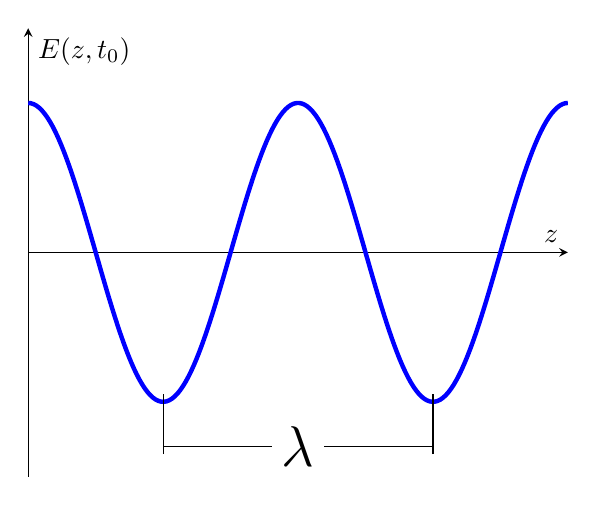
\begin{tikzpicture}
            \begin{axis}[
            axis x line=middle,
            axis y line=middle,
            ymax=1.5,
            ymin=-1.5,
            xmin=0,xmax=pi*4,
            xlabel= $z$,
            ylabel={$E(z,t_0)$},
            yticklabels={,,},
            xticklabels={,,},
            xtick=\empty,
            ytick=\empty,
            ]
            \addplot[domain=0:4*pi,samples=200,blue,ultra thick]{cos(deg(x))};
            \draw (pi,-1.35) -- (pi,-0.95);
            \draw (pi*3,-1.35) -- (pi*3,-0.95);
            \draw (pi,-1.3) -- (pi*3,-1.3) 
            node[pos=.5, fill=white,font=\huge] {$\lambda$};
            \end{axis}
        \end{tikzpicture}        
    \end{center}
    \caption{Plot of E in space}\label{fig:plot_E_space}
\end{figure}

\begin{figure}[H]
    \begin{center}
        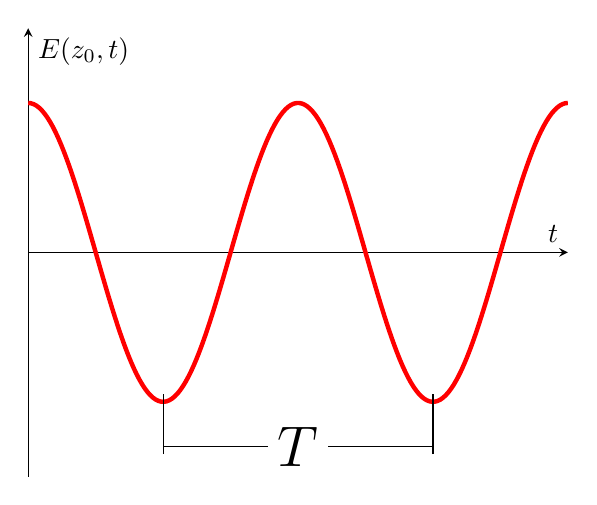
\begin{tikzpicture}
            \begin{axis}[
            axis x line=middle,
            axis y line=middle,
            ymax=1.5,
            ymin=-1.5,
            xmin=0,xmax=pi*4,
            xlabel= $t$,
            ylabel={$E(z_0,t)$},
            yticklabels={,,},
            xticklabels={,,},
            xtick=\empty,
            ytick=\empty,
            ]
            \addplot[domain=0:4*pi,samples=200,red,ultra thick]{cos(deg(x))};
            \draw (pi,-1.35) -- (pi,-0.95);
            \draw (pi*3,-1.35) -- (pi*3,-0.95);
            \draw (pi,-1.3) -- (pi*3,-1.3) 
            node[pos=.5, fill=white,font=\huge] {$T$};
            \end{axis}
        \end{tikzpicture}        
    \end{center}
    \caption{Plot of E in time} \label{fig:plot_E_time}
\end{figure}
We can plot the solution in \cref{eq:maxwell_solution_simple} by considering one of the two variable constant.
\begin{itemize}
    \item \textbf{\cref{fig:plot_E_space}}: if we assume constant time (like if you would take a photograph to the wave) we are evaluating the propagation in space, and so we can obtain the wavelength $\lambda$
    \item \textbf{\cref{fig:plot_E_time}}: if we assume constant space (like if you look the wave from a fixed position) we are evaluating the propagation in space, and so we can obtain the period $T$ 
\end{itemize} 
\subsubsection*{Speed of the wave}
As we said if we plot $E$ in constant time (\cref{fig:plot_E_space}) it is like to take a picture of the wave. If we evaluate the same plot, but in another time point, we can notice that the points of the wave has changed position \cref{fig:plot_E_variation}.\\
From the variation of the space in time we can evaluate the speed of the $E$ wave.
\begin{figure}[H]
    \begin{center}
        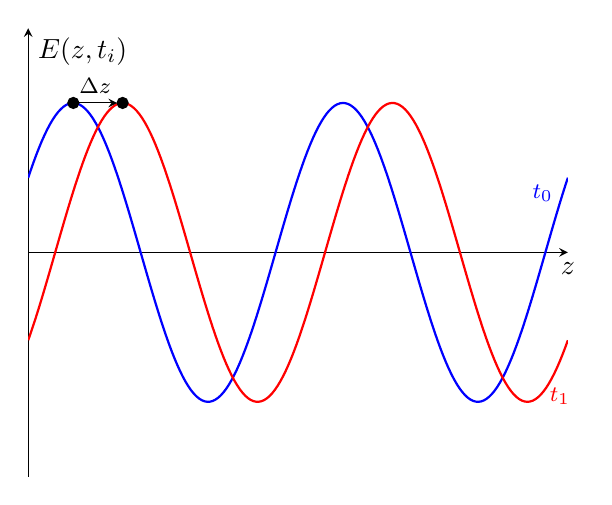
\begin{tikzpicture}
            \begin{axis}[
            axis x line=middle,
            axis y line=middle,
            ymax=1.5,
            ymin=-1.5,
            xmin=0,xmax=pi*4,
            x label style={anchor=north},
            xlabel= $z$,
            ylabel={$E(z,t_i)$},
            yticklabels={,,},
            xticklabels={,,},
            xtick=\empty,
            ytick=\empty,
            ]
            \addplot[domain=0:4*pi,samples=200,blue,thick]{cos(deg(x-pi/3))}
            node[left,pos=.99,font=\footnotesize]{$t_0$};
            \addplot[domain=0:4*pi,samples=200,red,thick]{cos(deg(x-pi*2.1/3))}
            node[right,pos=.95,font=\footnotesize]{$t_1$};
            \addplot [only marks] table {
                2.198 1
                1.05 1
                };
            \draw [stealth-](2.07,1) -- (1.05,1)
            node[midway, above,font=\footnotesize] {$\Delta z$};
            \end{axis}
        \end{tikzpicture}        
    \end{center}
    \caption{Plot of E in two different time}\label{fig:plot_E_variation}
\end{figure}
If we look at \cref{fig:plot_E_variation}, we can assumed that a point of the wave as moved from $z_1$ to $z_2$ from the instant $t_1$ to $t_2$. The function in the two points $(z_1,t_1)$ and $(z_2,t_2)$ has the same relative position (consider to "sit in the wave", you would feel like not moving, but the world around you is moving with a certain speed). So we can write:
\begin{align}
    \begin{split}
        &\omega\left(t_1-\frac{z_1}{c}\right)=\omega\left(t_2-\frac{z_2}{c}\right)\\[5pt]
        &t_2-t_1=\frac{z_2-z_1}{c}\\[5pt]
        &\Delta t= \frac{\Delta z}{c}\\[5pt]
        &c=\frac{\Delta z}{\Delta t}=\frac{\lambda}{T}
    \end{split}
\end{align}
We obtained the propagation speed of the wave:
\begin{equation}
    c=\frac{\partial z}{\partial t}=\frac{1}{\sqrt{\mu \varepsilon}}
\end{equation}
Note that the propagation speed is dependent of $\mu$ and $\varepsilon$, so we can calculate the speed in the vacuum:
\begin{equation}
    c_0=\frac{1}{\sqrt{\mu_0 \varepsilon_0}}=\frac{1}{\sqrt{\frac{1}{36\pi}\cdot 10^{-9}\cdot 4\,\pi\cdot 10^{-7}}}\approx 3\cdot 10^{8}[m/s]
\end{equation}
What we have found is a forward speed because $\Delta z$ is positive and $c$ positive, if we would have used the second equation from \cref{eq:maxwell_solution_simple} the space path $\Delta z$ need to be negative, or we would not be able to have a solution if we try to calculate the propagation speed:
\begin{equation}
    \omega\left(t_1+\frac{z_1}{c}\right)=\omega\left(t_2+\frac{z_2}{c}\right)
\end{equation}
\subsubsection*{Going back to the EMF}
Some more consideration of the EMF
\begin{equation}
    E(z,t)=E_0\,\cos(\omega t-\frac{\omega\,z}{c})
\end{equation}
Now we give some notation for:
\begin{itemize}
    \item $\bm{E_0}$ is the amplitude of the field.
    \item $\bm{\omega=2\,\pi\,\nu } $ is the angular frequency of the EMF
    \item $\bm{\nu =\frac{1}{T}}$ is the frequency of the EMF
\end{itemize}
We can also introduce the phase constant $\bm{\beta=\frac{\omega}{c}}$, and now the wave equation becomes:
\begin{equation}\label{eq:E_with_phase_constant}
    E(z,t)=E_0\cos(\omega\, t-\beta\,z)
\end{equation}
Those two parameters $\omega$ and $\beta$ are useful to obtain the propagation speed.\\
As we have done before, we "take a photo" of the wave (now $\omega t=constant$)and evaluated the propagation speed by considering $(\omega \,t-\beta \,z)$ to be constant, then:
\begin{equation}\label{eq:speed_of_EMF}
    \frac{\partial z}{\partial t}= \frac{\partial }{\partial t}\left(\frac{\omega t}{\beta}\right) = \frac{\omega}{\beta}
\end{equation}
\subsubsection*{Generalization of the EMF}
We can generalize a bit the EMF equation by adding an attenuation constant $\alpha$ and a reference phase $\varphi$
\begin{equation}\label{eq:wave_equation_generalized}
    E(z,t)=E_0\,e^{-\alpha\,z}\cos(\omega\,t-\beta\,z+\varphi)
\end{equation}
$\alpha$ is used to show how the wave is attenuated during his path on the medium.
\subsubsection*{EMF over a general direction}
Usually we consider $\khat$ as the direction of the EMF, but sometimes we need to generalize this direction over all the axes.\\
Consider the forward equation of the EMF over the 3 direction:
\begin{align}\label{eq:electric_field_3_axes}
    \begin{split}
        E(x,t)&=E_0\,\cos(\omega\,t-\beta_x\,x)\\[5pt]
        E(y,t)&=E_0\,\cos(\omega\,t-\beta_y\,y)\\[5pt]
        E(z,t)&=E_0\,\cos(\omega\,t-\beta_z\,z)
    \end{split}
\end{align}
What we do now is to find a way to merge those equation and describe the EMF that goes in a general direction $\overline{r}=x\,\ihat+y\,\jhat+z\,\khat$.\\
In order to do this we introduce the vector $\overline{k}=k_x\,\ihat+k_y\,\jhat+k_z\,\khat$ that generalize the $\beta$ factor, so we can write the wave equation with a general direction:
\begin{equation}
    E(\overline{r},t)=\overline{E}_0\,\cos(\omega\,t-\overline{k}\cdot\overline{r})
\end{equation}
Keep in mind that the direction is not $\overline{r}$ but $\overline{k}$, because $\overline{r}$ represent the variables, and $\overline{k}$ the three weights that defines the direction of the wave.
This is also called the plane wave equation, why?\\
Because we consider $\varphi = 0$ and $\omega\,t=0$ (we take a photo of the wave in $t=0$), so the wave fronts (where E is constant) can be obtained with:
\begin{equation}
    \cancel{\omega\,t}-\overline{k}\cdot\overline{r}+\cancel{\varphi}=-\overline{k}\cdot\overline{r}=k_x\,\ihat+k_y\,\jhat+k_z\,\khat=constant
\end{equation}
Then the last part of the equation is the equation of a plane.\\
Another thing that we can say, is that if $k$ is a scalar value, and $k\,\overline{r}$ is constant, the front of the wave have the shape of a sphere.
\section{Class 3 - 1/03/21}
During this class we will talk about the passage from the time domain to frequency. We do that because in frequency domain we do not need anymore to do the derivate in time, and thus the calculations simplify a lot. Another reason is that is more important to look at the signal on the corner frequency other than all over the spectrum
\subsection*{EMF in phasor domain}
Now we take a look at the electrical field propagating on the $z$ axe: $\overline{E}(z,t)=E_x\,\jhat+E_y\,\ihat+E_z\,\khat$, and we explore all the element:
\begin{align}\label{eq:electric_field_3_axes_phase}
    \begin{split}
        E_x(z,t)&=E_{x_0}\,\cos(\omega\,t-\beta\,z+\varphi_x)\\[5pt]
        E_y(z,t)&=E_{y_0}\,\cos(\omega\,t-\beta\,z+\varphi_y)\\[5pt]
        E_z(z,t)&=E_{z_0}\,\cos(\omega\,t-\beta\,z+\varphi_z)
    \end{split}
\end{align}
Note that here $\omega$ and $\beta$ does not change, but $\varphi$ does, this is not very important, but it is just a note.\\
From \cref{eq:electric_field_3_axes_phase}, and exploiting the cos property:
\begin{equation*}
    \cos(\alpha + \beta )=\cos\alpha\, \cos\beta - \sin\alpha \, \sin\beta
\end{equation*}
By considering $\alpha = \omega\, t$ and $\beta = \beta z+\varphi+z$ we obtain the total equation of the EMF on $z$ direction:
\begin{align}
    \begin{split}
        &\overline{E}(z,t)=E_x\,\jhat+E_y\,\ihat+E_z\,\khat=\\[5pt]
        &=\cos(\omega\,t)[E_{x_0}\cos(\varphi-\beta\,z)\ihat+E_{y_0}\cos(\varphi_y-\beta\,z)\jhat+E_{z_0}\cos(\varphi_z-\beta\,z)\khat]+\\[5pt]
        &-\sin(\omega\,t)[E_{x_0}\sin(\varphi-\beta\,z)\ihat+E_{y_0}\sin(\varphi_y-\beta\,z)\jhat+E_{z_0}\sin(\varphi_z-\beta\,z)\khat])=\\[5pt]
        &=\overline{E}_1\,\cos(\omega\,t)+\overline{E}_2\,\sin(\omega\,t)
    \end{split}
\end{align}
First of all we notice that $\overline{E}_1$ and $\overline{E}_2$ are vectors that are only in function of space (and that is great and useful).\\
Then we can write:
\begin{equation}
    \overline{E}(z,t)=\operatorname{Re}\left\{(\overline{E}_1+j\overline{E}_2)[\cos(\omega t)+j \sin(\omega t)]\right\}=\operatorname{Re}\left\{(\overline{E}_1+j\overline{E}_2)e^{j\omega t}\right\}
\end{equation}
With this notation we can introduce the phasor 
\begin{equation}
\phas{E}(z)=\overline{E}_1+j\overline{E}_2
\end{equation}
And we will use this notation to describe the EMF in complex notation.
\begin{equation}\label{eq:electric_field_in_time}
    \overline{E}(z,t)=\operatorname{Re}\left\{\phas{E}(z)e^{j\omega t}\right\}
\end{equation}
If we want to go from time domain to phasor, we need to find $E_1$ and $E_2$. To do the opposite we need to use \cref{eq:electric_field_in_time}.\\
Now let's give a look at the derivative of the field:
\begin{equation}
    \frac{\partial\overline{E}(z,t)}{\partial t}=\operatorname{Re}\left\{\frac{\partial}{\partial t}\phas{E}e^{j\omega t}\right\}=\operatorname{Re}\left\{j\omega\,\phas{E}e^{j\omega t}\right\}
\end{equation}
With this trick we can use the derivative by only multiplying $j\omega$.\\
That being said, we can give the definition of electric or magnetic field that propagates in a general direction:
\begin{align}
    \begin{split}
        &\overline{E}(\overline{r},t)=\operatorname{Re}\left\{\phas{E}(\overline{r})e^{j\omega t}\right\}\\[5pt]
        &\overline{H}(\overline{r},t)=\operatorname{Re}\left\{\phas{H}(\overline{r})e^{j\omega t}\right\}\\[5pt]
    \end{split}
\end{align}
Now in phasor domain, we can write the maxwell equations that we have already seen in \cref{eq:maxwell_system_2}, but with a simpler notation.
\begin{align}\label{eq:maxwell_equation_in_phasor}
    \begin{split}
        &\nabla\times\phas{E}=j\omega \,\phas{B}\\[5pt]
        &\nabla\times\phas{H}=j\omega \,\phas{D}+\phas{J}_\sigma+\phas{J}_i\\[5pt]
    \end{split}
\end{align}
Obviously this is true for any general direction $\overline{r}$, evn if we didn't mentioned that for a better notation elegance.\\
Another important thing that we need to stress is the relation of the other vectors that can be represented in the phasor space:
\begin{center}
    \begin{tabular}{ c c c }
        $\phas{D}=-\varepsilon \phas{E}$&
        $\phas{B}=\mu \phas{H}$&
        $\phas{J}_\sigma=\sigma\phas{E}$
    \end{tabular}
\end{center}
Note that $\varepsilon$,$\mu$ and $\sigma$ in this case are dependent on the position and frequency (not in time as before).
\begin{align}
    \begin{split}
        &\varepsilon=\varepsilon(\overline{r},\omega)\\[5pt]
        &\mu=\mu(\overline{r},\omega)\\[5pt]
        &\sigma=\sigma(\overline{r},\omega)
    \end{split}
\end{align}
\subsubsection*{Note on the refraction index}
The refraction index can become useful next, here we only introduce it and say what does it mean.\\
First of all we define refraction index $n$ as the square root of $\varepsilon_r$
\begin{equation}
    n=\sqrt{\varepsilon_r}=\sqrt{\frac{\varepsilon}{\varepsilon_0}}
\end{equation}
Actually this is a simplified relation, it is better to define $n$ as:
\begin{equation}
    n=\sqrt{\varepsilon_r\,\mu_r}=\sqrt{\frac{\varepsilon\,\mu}{\varepsilon_0\,\mu_0}}
\end{equation}
We already seen before that $c=\frac{1}{\sqrt{\varepsilon_0\,\mu_0}}$ and $v_p=\frac{1}{\sqrt{\varepsilon\,\mu }}$, so we the refraction index is very useful to describe the speed of an EMF through a medium:
\begin{equation}
    n=\frac{c}{v_0}
\end{equation}
\subsubsection*{Wave equation in phasor domain}
Given the system of equation in \cref{eq:maxwell_equation_in_phasor}, and applying some substitution we can obtain:
\begin{align}\label{eq:maxwell_equation_in_phasor_2}
    \begin{split}
        &\nabla\times\phas{E}=-j\omega\mu\,\phas{H}\\[5pt]
        &\nabla\times\phas{H}=j\omega \varepsilon\,\phas{E}+\sigma\phas{E}_\sigma+\overline{J}_i\\[5pt]
    \end{split}
\end{align}
It is evident that without derivative it is much more simple to find the wave equation.\\
For the sake of simplicity we will not make all the calculation to arrive to the final value, instead we use the old wave equation in time domain (\cref{eq:whave_2}) and we obtain the new wave equation in phasor domain:
\begin{equation}\label{eq:Helmholtz1}
    \nabla^2\,\phas{E}-\frac{\omega^2}{c^2}\,\phas{E}=0
\end{equation}
If we assume $E$ as a scalar field, then:
\begin{equation}\label{eq:Helmholtz2}
    \frac{\partial^2\phas{E}(z)}{\partial z^2}\nabla^2\,-\frac{\omega^2}{c^2}\,\phas{E}(z)=0
\end{equation}
\cref{eq:Helmholtz1} and \cref{eq:Helmholtz2} are also known as the Helmholtz equation (strange name, i know).
\subsubsection*{Solution of the wave equation in phasor domain}
Given \cref{eq:Helmholtz2}, it is very simple to obtain its solution.\\
Before to do that we introduce the parameter $\gamma$ such that:
\begin{equation}\label{eq:gamma_1}
    \gamma^2=-\frac{\omega^2}{c^2}=-\omega\,\mu\,\varepsilon
\end{equation}
Substituting $-\frac{\omega^2}{c^2}$ with $gamma$ from \cref{eq:Helmholtz2} we are able to get a possible solution:
\begin{equation}\label{eq:maxwell_solution_phasor1}
    \phas{E}=\overline{E}_{0_1}\,e^{\gamma z}+\overline{E}_{0_2}\,e^{-\gamma z}
\end{equation}
We know that $\gamma$ is a complex number because both $\mu$ and $\varepsilon$ are so:
\begin{equation}
    \gamma=\alpha+j\beta
\end{equation}
So we can write \cref{eq:maxwell_solution_phasor1} as:
\begin{equation}\label{eq:maxwell_solution_phasor}
    \phas{E}=\overline{E}_{0_1}\,e^{\alpha z}\,e^{j\beta z}+\overline{E}_{0_2}\,e^{-\alpha z}\,e^{-j\beta z}=
\end{equation}
We will focus on the forward wave equation $\phas{E}=\overline{E}_{0}\,e^{-\alpha z}\,e^{-j\beta z}$.
\subsubsection*{Going back from phasor to time domain}
If we want to go back to time domain from \cref{eq:maxwell_solution_phasor} we can just apply the relation from \cref{eq:electric_field_in_time}:
\begin{align}
    \begin{split}
        &\overline{E}(z,t)=\operatorname{Re}\left\{\phas{E}(z)e^{j\omega t}\right\}=\\[5pt]
        &=\operatorname{Re}\left\{\overline{E}_{0_2}\,e^{-\alpha z}\,e^{-j\beta z}e^{j\omega t}\right\} =\\[5pt]
        &=\operatorname{Re}\left\{|E_{0_2}|\,e^{j\varphi_0}\,e^{-\alpha z}\,e^{-j\beta z}e^{j\omega t}\right\} =\\[5pt]
        &= |E_{0_2}| e^{-\alpha z}\operatorname{Re}\left\{e^{j(\omega t-\beta z +\varphi_0)}\right\}=\\[5pt]
        &= |E_{0_2}| e^{-\alpha z}\operatorname{Re}\left\{\cos(\omega t-\beta z +\varphi_0)+j \sin(\omega t-\beta z +\varphi_0)\right\}=\\[5pt]
        &= |E_{0_2}| e^{-\alpha z}\,\cos(\omega t-\beta z +\varphi_0)
    \end{split}\label{eq:from_phas_to_time}
\end{align}
We obtained the forward equation of an EMF that propagates over the $z$ direction, that we have already seen in \cref{eq:wave_equation_generalized}.
\subsubsection*{Why $\varphi$ is a complex number?}
Consider the Maxwell equation in \cref{eq:maxwell_equation_in_phasor_2}, but without the $\overline{J}_i$ term (no current that is generating the EMF).\\
I'll not write again the \cref{eq:maxwell_equation_in_phasor_2} because you can find it simply clicking at the reference number, that being said we can do something with the second relation:
\begin{align}
    \begin{split}
        &\nabla\times\phas{H}=j\omega \varepsilon\,\left(1+\frac{\sigma}{j\omega \epsilon}\right)\phas{E}=\\[5pt]
        &\nabla\times\phas{H}=j\omega \varepsilon\,\left(1-j\frac{\sigma}{\omega \epsilon}\right)\phas{E}=\\[5pt]
        &\nabla\times\phas{H}=j\omega \underbrace{\varepsilon\,\left(1+\frac{\sigma}{j\omega \epsilon}\right)}_{\varepsilon_c}\,\phas{E}=\\[5pt]
        &\nabla\times\phas{H}=j\omega \varepsilon_c\,\phas{E}\\[5pt]
    \end{split}
\end{align}
$\varepsilon_c$ is the complex permittivity, with this the maxwell equation becomes very similar to \cref{eq:maxwell_simplified}:
\begin{equation}\label{eq:maxwell_equation_in_phasor_simplified}
    \begin{cases}
    \nabla\times\phas{E}=-j\omega\,\mu \phas{H}\\[5pt]
    \nabla\times\phas{H}=\;\;\,j\omega \, \varepsilon_c\phas{E}
    \end{cases}
\end{equation}
So \cref{eq:gamma_1} is not totally correct because we need to consider the complex permittivity $\varepsilon_c$: $\gamma^2=-\omega\,\mu\,\varepsilon_c$.\\
An interesting thing to note is that the imaginary part of $\varepsilon_c=\varepsilon\,\left(1-j\frac{\sigma}{\omega \epsilon}\right)$ are the losses during the propagation of the EMF through a medium
\begin{itemize}
    \item $\bm{\sigma}$: metallic medium loss
    \item $\bm{\omega \epsilon}$: dielectric medium loss
\end{itemize}
We can also use $\frac{\sigma}{\omega \epsilon}$ to know the property of our medium:
\begin{itemize}
    \item $\bm{\frac{\sigma}{\omega \epsilon}> 1}$: metallic medium
    \item $\bm{\frac{\sigma}{\omega \epsilon}< 1}$: dielectric medium loss
\end{itemize}
If we suppose no metallic loss: $\sigma = 0$, then:
\begin{equation*}
    \theta=0\rightarrow\varepsilon_c=\varepsilon\rightarrow\alpha=0\rightarrow\gamma =j\beta
\end{equation*}
With this simplification the forward magnetic field becomes:
\begin{equation}
    \phas{E}=\overline{E}_{0}\, e^{-j\beta z}
\end{equation}
\subsection*{EMF in frequency domain}
Until now we have seen a pure sinusoidal EMF that propagates, what if this EMF is not pure?\\
We can say that our signal is not a pure sinusoid if we have more than 1 component other than the fundamental harmonic, this mean that we deal with noisy signal.\\
Similarly to \cref{eq:electric_field_in_time}, we can define the transformation from time domain to frequency domain as:
\begin{equation}
    \overline{E}(\overline{r},t)=\frac{1}{2\pi}\int_{-\infty}^{+\infty}\overline{E}(\overline{r},w)e^{j\omega t}
\end{equation}
That transformation is actually the same as the one for the complex domain, but we now can consider more than 1 harmonic.\\
Again here we don't deal anymore with derivatives in time, so our job simplify a lot!:
\begin{equation}
    \frac{\partial\overline{E}(\overline{r},t)}{\partial t}=\frac{1}{2\pi}\int_{-\infty}^{+\infty}j\omega\,\overline{E}(\overline{r},w)e^{j\omega t}
\end{equation}
Like in \cref{eq:maxwell_equation_in_phasor_simplified} we can have a look at the Maxwell equation in phasor domain again without the $\overline{J}_i$ term (no current that is generating the EMF).\\
You can notice that they are actually the same, but in frequency the field $E$ and $H$ are dependent in time and also in frequency.
\begin{align}
    \begin{split}
        &\nabla\times\overline{E}(t,\omega)=-j\omega\mu\,\overline{H}(t,\omega)\\[5pt]
        &\nabla\times\overline{H}(t,\omega)=\;\;\,j\omega \varepsilon\,\overline{E}(t,\omega)
    \end{split}
\end{align}
And the wave equation becomes:
\begin{equation}
    \nabla^2\,\overline{E}(t,\omega)-\gamma^2\,\overline{E}(t,\omega)=0
\end{equation}
\subsection*{A little exercise}
The prof said it was little... but i'm too tired to copy all the numbers, but here i reported the passages.\\
 The request was to find the expression of the EMF ($E$ and $H$ equation) given $\gamma $, the direction $z$ and supposing no losses ($\alpha=0$). The field of $E$ is on his peak $E_0$ wen $t=0$ and $z=50$\\
 First of all the peak of the field $E_0$ is obtained when $\cos(\omega t-\beta z +\phi_0)=1$, so when $(\omega t-\beta z +\phi_0)=0$.\\
 We can simplify saying that $\omega t =0$ (we can assume the initial time $t_0=0$ because of the given data).\\
 From \cref{eq:gamma_1} we can obtain $\omega$ from $\gamma$ ($\omega^2=c^2-\omega^2$).\\
 From \cref{eq:E_with_phase_constant} we also know that $\beta=\frac{\omega}{c}$.\\
Then we obtain $\varphi_0$ from $-\frac{\omega}{c}+\phi_0=0$.\\
We have all we need to write down the equation for $E$ in time
\begin{equation*}
    E(z,t)=E_0\, \cos(-\beta z +\phi_0)\,\ihat
\end{equation*}
What about $H$?
\begin{equation}
    \nabla\times \overline{E}=\frac{\partial E_x}{\partial z}\jhat=-\mu\frac{\partial \overline{H}}{\partial t}\jhat
\end{equation}
Doing some strange calculation we can obtain the $H$ equation, where the argument of $cos$ are the same, but $H_0$ changes:
\begin{equation*}
    H(z,t)=H_0\, \cos(-\beta z +\phi_0)\,\jhat
\end{equation*}
\subsubsection*{Frequency domain}
In frequency it is much more simple:
\begin{equation*}
    \phas{E}(z)=\overline{E_0}\,\cancelto{0}{e^{-\alpha z}}\,e^{-j\beta z}=|E_0|\,e^{-j\beta z}\,e^{j\varphi_0}
\end{equation*}
We already have $E_0$, $\beta$ and $\varphi_0$ can be simply calculated as before.\\
Now $\phas{H}(z)$??
\begin{align}
    \begin{split}
        &\frac{\partial \phas{E_x}}{\partial z}=-j\omega\mu\,\phas{H}\\[5pt]
        &\phas{H}=\frac{1}{-j\omega\mu}\frac{\partial \phas{E_x}}{\partial z}=\\[5pt]
        &=\frac{j}{\omega \beta}\overline{E_0}e^{-j\beta z}=\\[5pt]
        &=\frac{\beta}{\mu \omega}|E_0|\, e^{j\varphi_0}e^{-j\beta z}
    \end{split}
\end{align}
We know that $\beta = \frac{\omega}{c}$, then we obtain the intrinsic impedance $\eta$:
\begin{equation}\label{eq:intrinsic_impedance}
    \frac{\omega}{c}\,\frac{1}{\omega \mu}=\frac{\sqrt{\mu \varepsilon}}{\mu}=\sqrt{\frac{\epsilon}{\mu}}=\eta 
\end{equation}
So we obtain a very useful equation:
\begin{equation}
    \phas{H}=\frac{1}{\eta}\,\overline{E_0}e^{-j\beta z}
\end{equation}
And we can also say that if the field propagates along $z$:
\begin{align}\label{eq:useful_maxwell_in_phasor}
    \begin{split}
        \phas{H}&=\frac{1}{\eta}\,\khat \times \phas{E}\\[5pt]
        \phas{E}&=\eta\,\phas{H}\times \khat
    \end{split}
\end{align}
Note that the second equation in \cref{eq:useful_maxwell_in_phasor} is very similar to the first hom law because we have:
\begin{equation*}
    \left[\frac{V}{m}\right]=\eta\,\left[\frac{A}{m}\right]
\end{equation*}
Just like $\left[V\right]=\Omega \,\left[A\right]$
\subsection*{One more thing: Poynting vector}
The \emph{Poynting vector} represents the directional energy flux of our radiation, this mean that it is not simply the "representation" of the power density of an EMF, but we also have the direction of the propagating wave, and it is defined by:
\begin{equation}\label{eq:poynting}
    \overline{S}=\overline{E}\times\overline{H}\rightarrow\left[\frac{w}{m^2}\right]
\end{equation}
To obtain $\overline{S}$ is not very simple, but in phasor domain it is \emph{na crema} (italian way to say "very beautiful"):
\begin{equation}
    \overline{S}=\frac{\phas{E}\times\phas{H}^*}{2}=\frac{1}{2}\,\overline{E}
_x\cdot\overline{H}_y^*\,\khat
\end{equation}
\section{Class 4 - 5/03/21}
\subsection*{Transmission line}
When we have a signal to be transmitted over a cable, the problem to connect the source of the signal to the load is not as simple as cabling a dc power source. In our case the voltage level to be transmitted can be considered as a wave, and his behavior over the transmission line can vary with the length, the frequency of the signal or also with the geometry of the cable.
\begin{figure}[H]
\begin{center}
    \begin{circuitikz} [ baseline=(current bounding box.center)]
        \ctikzset { label/align = straight }
        \node[draw,minimum width=4cm,minimum height=2.4cm,anchor=south west] at (2.5,-0.2){TL};
        \draw (0,0)
        to[sV=$V_{g}$] (0,2)
        to[R=$R_{g}$, -o] (2,2)
        node[label={[font=\footnotesize]above:$A$}] {}
        to[short] (2.5,2)
        (0,0) to[short, -o] (2,0) 
        node[label={[font=\footnotesize]below:$A'$}] {}
        to[short] (2.5,0);
        \draw (8.5,0) 
        to[short, -o] (7.,0)
        node[label={[font=\footnotesize]below:$B'$}] {}
        to[short](6.5,0)
        (8.5,2) to[generic=$Z_{l}$] (8.5,0)
        (8.5,2) to[short, -o] (7,2)
        node[label={[font=\footnotesize]above:$B$}] {}
        to[short](6.5,2)
        ;
      \end{circuitikz}     
\end{center} \caption{Transmission line example} \label{fig:transmission_line_example}
\end{figure}
In \cref{fig:transmission_line_example} a very simplified view of a transmission line, where the voltage at the input is the one over $AA'$, and $BB'$ on the output.\\
If we do not consider the resistance $R_g$, then the voltage in input of the TL can be seen as:
\begin{equation}
  V_{AA'}(t)=V_g(t)=V_0 \, \cos(\omega t)
\end{equation}
Now for the output voltage equation we need to consider the time delay of signal travelling from $A$ to $B$. So we need to consider the same signal $V_{AA'}$ but delayed by $\frac{l}{c}$ ($l$ is the length of the TL, and $c$ is the speed of the signal, the same speed of light).
\begin{align}\label{eq:vbb_in_transmission_line}
  \begin{split}
    V_{BB'}(t)&=V_{AA'}\left(t-\frac{l}{c}\right)=\\[5pt]
      &=V_0 \, \cos\left[\omega \left(t-\frac{l}{c}\right)\right]=\\[5pt]
      &=V_0\, \cos\left(\omega t-\frac{\omega}{c}\, l\right)=\\[5pt]
      &=V_0\, \cos\left(\omega t-\beta\, l\right)= \\[5pt]
  \end{split}
\end{align}
Actually in \cref{eq:vbb_in_transmission_line} we can see that our signal over the transmission line is actually a wave dependent on the frequency and the length of the cables.
\subsection*{Example on different transmission line length}
As we can see in \cref{eq:vbb_in_transmission_line}, we need to face a new problem: how the strength of our signal change accordingly to the length of my transmission line?\\
For example, on the input of the TL we have a signal with amplitude $A_0$ and a frequency of $f=\SI{1}{\kilo\hertz}$.\\
Suppose the length of the TL $l=\SI{5}{\centi \meter}$, then the signal on the output at $t=0$ will be:
\begin{align*}
  \begin{split}
  V_{BB'}(t)&=V_0\, \cos\left(\omega t-\beta\, l\right)=\cos\left(\omega t-\frac{\omega}{c}\, l\right)=\\[5pt]
  &=V_0\, \cos\left(2\,\pi\,10^{3}\cdot 0+\frac{2\,\pi\,10^{3}}{3\cdot 10^{8}}\cdot 0.05\right)=\\[5pt]
  &=V_0\,\cos(0,105 \cdot 10^{-5})\approx V_0\cdot 0.999\approx V_0
  \end{split}
\end{align*}
As we can see, we have a very short length of the cable compared to the wavelength, the attenuation over the line due is totally negligible.\\
If we suppose instead the length of the TL: $l=\SI{100}{\kilo \meter}$, then the signal on the output at $t=0$ will be:
\begin{align*}
  \begin{split}
  V_{BB'}(t)&=V_0\, \cos\left(2\,\pi\,10^{3}\cdot 0+\frac{2\,\pi\,10^{3}}{3\cdot 10^{8}}\cdot100\cdot 10^{3}\right)=\\[5pt]
  &=V_0\,\cos(2.09)\approx V_0\cdot -0.49\approx -\frac{1}{2}\,V_0
  \end{split}
\end{align*}
It is very important to notice that now the amplitude of the signal is half as before, just by moving away from the source, and without considering the attenuation of the line.\\
This behavior can be explained by looking at the argument of the $cos$ on \cref{eq:vbb_in_transmission_line}: 
\begin{itemize}
  \item $\bm{(\omega t)}$ : is responsible to the information propagation (otherwise we could not detect the wave).
  \item $\bm{(\beta\, l)}$ : is the one dependent on the length that we need to investigate.
\end{itemize}
What we can notice is that the effect of that attenuation depends a lot on the wavelength:
\begin{equation*}
  \beta\, l=\frac{\omega}{c}\,l=\frac{2\pi}{c}\cdot f\cdot l=2\pi\cdot\frac{l}{\lambda}
\end{equation*}
The cosine operator is periodic over $2\pi$, this mean that when the length of the TL $l$ is a multiple of the wavelength $\lambda$, the output signal won't be attenuated: $\cos(k\,2\pi)=1$.\\
But when $l = (\frac{n}{2}+1)\,\lambda$ for $n=0,1,\cdots$ at $t=0$, on the output of the TL we will not see any signal because $\cos(k\,\frac{\pi}{2})=1$\\
Now you could say: \textit{"hey!, that sounds like a simple phase shift, we can just wait $\frac{\pi}{2}$ and then the signal amplitude will be again $A_0$"}, that is true my friend, but by this example it is very simple to understand how a signal can change if we move over a transmission line.\\
In the next section we will talk about a real attenuation of the signal along the TL (for example we will be able to choose the right distance from the source to guarantee the maximum power transfer).\\
Another thing that we will take in consideration is the losses over the line, and the attenuation of the reflected signal.
\subsubsection*{How can we model our transmission line?}
To propagate an electric signal we need 2 conductors, it is not important if they are twisted pairs or coaxial (for now).\\
Then we can divide our line in different sectors of length $\Delta z$, and each segment can be modelled as a circuit:
\begin{figure}[H]
  \begin{center}
      \begin{circuitikz} [ baseline=(current bounding box.center)]
          \ctikzset { label/align = straight }
          \draw (8,0)
          to[short, o-o,] (0,0)
          (0,4)
          to[R=$R\,\Delta z$,o-] (2,4)
          to[L=$L\,\Delta z$] (4,4)
          to[short,-o](8,4)
          (4,4)to[short](4,3)
          (3,3)to[short](5,3)
          (3,1)to[short](5,1)
          (4,0)to[short](4,1)
          (5,3)to[C=$C\,\Delta z$](5,1)
          (3,1)to[R=$G\,\Delta z$](3,3)
          ;
          \draw [decorate,decoration={brace,amplitude=6pt,mirror,raise=1ex}]
          (0,0) -- (8,0) node[midway,yshift=-2em]{$\Delta z$};
        \end{circuitikz}     
  \end{center} \caption{Circuital representation of a TL section} \label{fig:transmission_section_delta_z}
\end{figure}
Now from \cref{fig:transmission_section_delta_z} we can see different parameters:
\begin{itemize}
  \item $\bm{R\,\Delta z}$ : Resistance representing the losses on both conductors along the line.
  \item $\bm{L\,\Delta z}$ : Inductive behavior of the cable.
  \item $\bm{G\,\Delta z}$ : Conductance representing the losses due to the separator.
  \item $\bm{C\,\Delta z}$ : Capacitive behavior due to the two conductors.
\end{itemize}
\subsubsection*{Example of coaxial conductor}
\begin{figure}[H]
    \begin{center}
    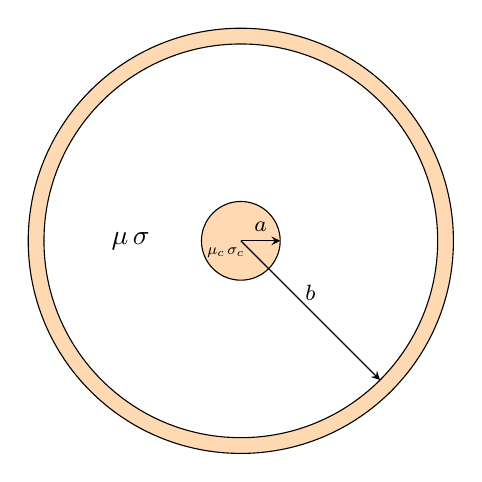
\begin{tikzpicture}
      \coordinate (O) at (0,0);
      \draw [fill=orange!30](O) circle (2.7);
      \draw  [fill=white](O) circle (2.5);
      \draw [fill=orange!30](O) circle (0.5);
      \draw[stealth-](0.5,0) -- (0,0)
      node[midway, above,font=\footnotesize] {$a$};
      \draw[stealth-](1.76775,-1.76775) -- (0,0)
      node[midway, above,font=\footnotesize] {$b$};
      \node (s) at (-1.4,0) {$\mu\,\sigma$};
      \node (s) [font=\footnotesize,scale=0.7] at (-0.19,-0.15) {$\mu_c\,\sigma_c$};
    \end{tikzpicture}  
  \end{center}\caption{Simplified coaxial section}
\end{figure}
The most common example of transmission line is the coaxial cable:\\
in our example we suppose the inner conductor radius $a$ and outer conductor radius $b$, then we also need to know the electric characteristic of the conductor ($\mu_c$ and $\sigma_c$) and the one of the separator ($\mu$ and $\sigma $). We can write now the characteristic value of the transmission line:
\begin{alignat*}{2}
    R&=\frac{R_s}{2\pi}\left(\frac{1}{a}+\frac{1}{b}\right)\;&&   \left[\si{\ohm\per\metre}\right]\\[5pt]
    L&=\frac{\mu}{2\pi}ln \left(\frac{b}{a}\right)&& \left[\si{\henry\per\metre}\right]\\[5pt]
    G&=\frac{2\pi\sigma}{ln\left(\frac{b}{a}\right)}&&\left[\si{\siemens\per\metre}\right]\\[5pt]
    C&=\frac{2\pi \epsilon}{ln\left(\frac{b}{a}\right)}&&\left[\si{\farad\per\metre}\right]
\end{alignat*}
$R_s$ is the resistance on the surface of the conductor and $R_s=\sqrt{\frac{\pi f \mu_c}{\sigma_c}}$.\\
Now let's make some consideration on $L$ and $C$:
\begin{equation}\label{eq:relation_LC_muepsilon}
  L\cdot C=\frac{\mu}{\cancel{2\pi}}\cancel{ln\left(\frac{b}{a}\right)}\frac{\cancel{2\pi}\,\varepsilon}{\cancel{ln\left(\frac{b}{a}\right)}}=\mu\cdot\varepsilon
\end{equation}
This relation $L\cdot C= \mu\cdot\varepsilon$ is very interesting for us, because we have already sen that $c=\frac{1}{\sqrt{\mu\,\varepsilon}}$ and $\beta=\omega\sqrt{\mu\,\varepsilon}$.\\
So what does the \cref{eq:relation_LC_muepsilon} mean? The answer is that when the EMF is forced to move inside a cable we will not use $\mu$ and $\varepsilon$, but $L$ and $C$, and that is very useful and cool for us.
\subsection*{Telegraph equations}
To obtain some cool relation for our TL we can use the Kirchhoff law as usual.
\begin{figure}[H]
  \begin{center}
      \begin{circuitikz} [ baseline=(current bounding box.center)]]
          \ctikzset { label/align = straight}
          \par\ctikzset{bipoles/resistor/width=.6,bipoles/resistor/height=.25}
          \draw (0,0)
          to[short, o-o,] (8,0)
          (0,4)to[short,i={$i(z,t)$},o-](1,4)
          to[R=$R\,\Delta z$] (2,4)
          to[L=$L\,\Delta z$] (4,4)
          to[short](7,4)
          to[short,i={$i(z+\Delta z,t)$},-o](8,4)
          (4,4)to[short](4,3)
          (3,3)to[short](5,3)
          (3,1)to[short](5,1)
          (4,0)to[short](4,1)
          (5,3)to[C=$C\,\Delta z$](5,1)
          (3,1)to[R=$G\,\Delta z$](3,3)
          (0,0)to[european voltages,open,v^={$v(z,t)$}](0,4)
          (8,0)to[european voltages,open,v_={$v(z+\Delta z,t)$}](8,4)
          (0,0) -- (8,0) node[midway,yshift=-1em]{$\Delta z$};
          ;
        \end{circuitikz}     
  \end{center} \caption{Circuital representation of a TL section with Kirchhoff}\label{eq:TL_with_kk}
\end{figure}
Now we can analyze the circuit in \cref{eq:TL_with_kk} using the Kirchhoff law:
\begin{equation*}
  v(z,t)-R\,\Delta z\,i(z,t)-L\,\Delta z\,\frac{\partial i(z,t)}{\partial t}=v(z+\Delta z,t)
\end{equation*}
Divide all for $\Delta z$
\begin{equation*}
  -\frac{v(z+\Delta z,t)-v(z,t)}{\Delta z}=R\,i(z,t)+L\,\frac{\partial i(z,t)}{\partial t}
\end{equation*}
Now let shrink the interval $\Delta z\rightarrow 0$
\begin{equation}\label{eq:Telegraph_eq}
  \begin{cases}
  -\frac{\partial v(z,t)}{\partial z}=R\,i(z,t)+L\frac{\partial i(z,t)}{\partial t}\\[5pt]
  -\frac{\partial i(z,t)}{\partial z}=G\,v(z,t)+C\frac{\partial v(z,t)}{\partial t}
  \end{cases}
\end{equation}
In \cref{eq:Telegraph_eq} we obtained the so called \emph{telegraph equations}.\\
The second equation in \cref{eq:Telegraph_eq} can be obtained by doing the same calculation that we have already done for the first one.\\
If we do not consider losses, those equations becomes even prettier:
\begin{equation}\label{eq:Telegraph_eq_prettier}
  \begin{cases}
  -\frac{\partial v(z,t)}{\partial z}=L\frac{\partial i(z,t)}{\partial t}\\[5pt]
  -\frac{\partial i(z,t)}{\partial z}=C\frac{\partial v(z,t)}{\partial t}
  \end{cases}
\end{equation}
\subsubsection*{Wave equation of the signal on the TL}
To obtain the wave equation, we can use the derivative over the space on the first equation of \cref{eq:Telegraph_eq_prettier}:
\begin{align}
  \begin{split}
  -\frac{\partial^2 v(z,t)}{\partial z^2}&=L\frac{\partial}{\partial t}\frac{\partial i(z,t)}{\partial z}\\[5pt]
  \frac{\partial^2 v(z,t)}{\partial z^2}&-L\,C\frac{\partial^2 v(z,t)}{\partial t^2}=0\\[5pt]
  \frac{\partial^2 v(z,t)}{\partial z^2}&-\frac{1}{c^2}\frac{\partial^2 v(z,t)}{\partial t^2}=0
  \end{split}\label{eq:wave_eq_on_TL}
\end{align}
The wave equation obtained in \cref{eq:wave_eq_on_TL} is very similar to what we have fond before, from here we can also obtain the solution of that equation:
\begin{equation}
  v(z,t)=V\bottomPlus \,\cos\left(\omega t-\frac{\omega}{c}z\right)+V\bottomMinus \,\cos\left(\omega t+\frac{\omega}{c}z\right)
\end{equation}
\subsubsection*{Telegraph and wave equation in phasor domain}
Starting from \cref{eq:Telegraph_eq_prettier} we can obtain the telegraph equation in phasor domain:
\begin{equation}
  \begin{cases}\label{eq:telegraph_in_phas_1}
  -\frac{\partial \phas{V}}{\partial z}=(R+j\omega L)\phas{I}\\[5pt]
  -\frac{\partial \phas{I}}{\partial z}=(G+j\omega C)\phas{V}
  \end{cases}
\end{equation}
Then the wave equation becomes:
\begin{align}
  \begin{split}
    &-\frac{\partial^2 \phas{V}}{\partial z^2}=(R+j\omega L)\frac{\partial \phas{I}}{\partial z}=\\[5pt]
    &=(R+j\omega L)(G+j\omega C)\phas{V}
  \end{split}
\end{align}
We introduce $\gamma = \sqrt{(R+j\omega L)(G+j\omega C)}=\alpha+j\beta$, then we obtain the telephone equation (another name for the wave equation for TL):
\begin{equation}
  \begin{cases}
  \frac{\partial^2 \phas{V}}{\partial z^2}-\gamma^2\,\phas{I}=0\\[5pt]
  \frac{\partial^2 \phas{I}}{\partial z^2}-\gamma^2\,\phas{V}=0
  \end{cases}\label{eq:telephone_eq}
\end{equation}
We can also write a beautiful solution from \cref{eq:telephone_eq}:
\begin{equation}\label{eq:voltage_in_phas_domain}
  \phas{V}(z)=V\bottomPlus \,e^{-\gamma z}+V\bottomMinus \,e^{\gamma z}
\end{equation}
We also know that $\gamma$ is a complex number, so what we can do is to write the same equation, but dividing $\gamma = \alpha+j\beta$ and looking only at the forward:
\begin{equation}
  \phas{V}(z)=V\bottomPlus \,e^{-\alpha z}\,e^{-j\beta z}
\end{equation}
If i go back to time domain (see \cref{eq:from_phas_to_time}):
\begin{equation}\label{eq:from_phas_to_time_TL}
  v(z,t)=V\bottomPlus e^{\alpha z}\cos(\omega t-\beta z)
\end{equation}
Inside $\gamma $ we have $R$,$L$,$G$ and $C$, so we have all the geometry and physical characteristic of the TL.
\subsubsection*{What could happen if we assume no losses?}
If we assume no losses over the line, then $\alpha=0$, and so $\gamma = j\beta$, then the wave propagation will follow \cref{eq:wave_solution_no_losses}:
\begin{equation}
  \begin{cases}
  \phas{V}(z)=V\bottomPlus \,e^{-j\beta z}+V\bottomMinus \,e^{j\beta z}=\phas{V_p}(z)+\phas{V_r}(z)\\[5pt]
  \phas{I}(z)=I\bottomPlus \,e^{-j\beta z}+I\bottomMinus \,e^{j\beta z}=\phas{I_p}(z)+\phas{I_r}(z)
  \end{cases}\label{eq:wave_solution_no_losses}
\end{equation}
So what are the parameters that give losses? We obtain the $\alpha$ and $\beta$ value from the real and imaginary value of:
\begin{align}
  \begin{split}
    \gamma &=\sqrt{(R+j\omega L)(G+j\omega C)}=\\[5pt]
    &=\sqrt{R\,G+j\omega L\,G+j\omega C\,R-\omega^2L\,C}=\\[5pt]
    &=\sqrt{j\omega( L\,G + C\,R)+R\,G-\omega^2L\,C}\\[5pt]
  \end{split}
\end{align}
I will not go further because i don't know how to do that, but the imaginary part is:
\begin{equation}
  \beta=\omega\sqrt{L\,C}
\end{equation}
\section{Class 5 - 08/03/21}
\subsection*{characteristic impedance}
We can start this lecture by computing the derivative over the space of the voltage equation in phasor domain in \cref{eq:voltage_in_phas_domain}.
\begin{equation}
    \frac{\partial \phas{V}(z)}{\partial z}=\gamma \cdot \left(-Z_i(l)\,e^{-\gamma z}+V\bottomMinus \,e^{\gamma z}\right) 
\end{equation}
Then from the first equation in \cref{eq:telegraph_in_phas_1} we can obtain another way to express the current in phasor domain:
\begin{equation}
    \phas{I}(z)=\overbrace{\frac{\gamma}{(R+j\omega L)}}^{\frac{1}{Z_0}}\left[V\bottomPlus \,e^{-\gamma z}-V\bottomMinus \,e^{\gamma z}\right]
\end{equation}
If we take a look on that equation, we can notice a very interesting pattern, that look like the ohm's law: $I=G\,V$ with $G$ the conductivity of the circuit, or the inverse of the resistivity.\\
If you look closely, also $\frac{\gamma}{(R+j\omega L)}$ is a conductance:
\begin{equation}
    \frac{\gamma}{(R+j\omega L)}=\frac{\sqrt{(R+j\omega L)\,(G+j\omega C)}}{(R+j\omega L)}=\sqrt{\frac{G+j\omega L}{R+j\omega C}}
\end{equation}
The inverse of that term is an impedance, and we call that \emph{characteristic impedance} (lol, what a fantasy, you should give pokemon's name):
\begin{equation}
    Z_0=\sqrt{\frac{R+j\omega L}{G+j\omega C}}\;\left[\Omega \right]
\end{equation}
Without losses, the same equation becomes:
\begin{equation} \label{eq:characteristic_impedance_no_loss}
    Z_0=\sqrt{\frac{j\omega L}{j\omega C}}=\sqrt{\frac{L}{C}}
\end{equation}
If you look closely, \cref{eq:characteristic_impedance_no_loss} is very similar to the intrinsic impedance $\eta = \sqrt{\frac{\mu}{\varepsilon}}$ (\cref{eq:intrinsic_impedance}).\\
The current and current expression becomes:
\begin{equation}
    \begin{cases}
    \phas{V}(z) = V\bottomPlus \,e^{-j\beta z}+V\bottomMinus \,e^{j\beta z} \\[5pt]
    \phas{I}(z)=\frac{1}{Z_0}\left[V\bottomPlus \,e^{-\gamma z}-V\bottomMinus \,e^{\gamma z}\right]
    \end{cases}\label{eq:current_and_voltage_in_TL_phas}
\end{equation}
From now on, sometimes i could miss some phasor notation over $V$ and $I$, this was very important to emphasize the difference between the different domains, but no the next pages if you see $V(l)$ or $I(l)$ just remember that those wave expression does not contain the time $t$, so they are in phasor domain.\\
That being said, we can also write:
\begin{align}
    \begin{split}
      &V\bottomMinus = - Z_0 \,I\bottomMinus \\[5pt]
      &V\bottomPlus = Z_0 \,I\bottomPlus 
    \end{split}
\end{align}

\subsection*{Input impedance}
\begin{figure}[H]
    \begin{center}
        \begin{circuitikz} [ baseline=(current bounding box.center)]
            \ctikzset { label/align = straight }
            \draw (0,3)
            node[label={[font=\normalsize]above:$in$}] {}
            to[short, o-o,] (7,3)
            node[label={[font=\normalsize]above:$out$}] {}
            to[short](8.5,3)
            to[generic=$Z_{l}$] (8.5,0)
            to[short](7,0)
            to[short, o-o,] (0,0)
            ;
            \draw [-|] (0,-0.5) -- (7,-0.5)
            node[label={[font=\large]below:$0$}] {}
            ;
            \draw [->] (7,-0.5) -- (9,-0.5)
            node[label={[font=\large]right:$l$}] {}
            ;
            \draw (4,1)node[label={[font=\LARGE]above:$Z_0$}] {}
            ;
          \end{circuitikz}     
    \end{center} \caption{Transmission line with reference system}\label{fig:general_transmission_line_ref}
  \end{figure}
We assume that our transmission line is like in \cref{fig:general_transmission_line_ref}, here you can see that we introduced a reference system on the length of the line. The new coordinate $l$ is increasing on the right, and the zero point is set on the output coordinate of the line.
Starting from the equation of the signal over the line (with no losses) in \cref{eq:wave_solution_no_losses}, we can obtain the \emph{input impedance} of the line dependent on the position $l$:
\begin{align}
    \begin{split}\label{eq:input_impedance}
      Z_i(l)&=\frac{\phas{V}(l)}{\phas{I}(l)}=\frac{V\bottomPlus \,e^{-j\beta z}+V\bottomMinus \,e^{j\beta z}}{I\bottomPlus \,e^{-j\beta z}+I\bottomMinus \,e^{j\beta z}}\\[5pt]
      &=Z_0\,\frac{V\bottomPlus \,e^{-j\beta z}+V\bottomMinus \,e^{j\beta z}}{V\bottomPlus \,e^{-j\beta z}-V\bottomMinus \,e^{j\beta z}}
    \end{split}
\end{align}
Note that $Z_i(l)$ and $Z_0$ are very different, the first one can depend on the position over the line. But we can notice an important relation between the two when we are in $l=0$:
\begin{equation}\label{eq:input_impedance_l=0}
    Z_i(l=0)=Z_L=\frac{V_L}{I_L}=Z_0 \,\frac{V\bottomPlus +V\bottomMinus }{V\bottomPlus -V\bottomMinus }
\end{equation}
\subsubsection*{To not make confusion!}
All this notation is very confusing in my opinion, so a fast clarification:
\begin{itemize}
    \item $Z_0$ is the characteristic impedance, it is the same for all the line and can be considered like the impedance of the tiny tiny section of the TL.
    \item $Z_i(l)$ is the impedance that you would measure if you take a very special oscilloscope in a specific position $l$ on your line.\\
    If you are in $l=0$ you are measuring the load ($Z_L$).\\
    If you are in $l=L$ you are measuring the impedance on the input side of the TL (also named input impedance), so what impedance your generator see ($Z_{in}$).
    \item $\phas{V}(l)$ is the voltage that you would measure if you take a special oscilloscope in a specific position $l$ on your line (in phasor domain).
    \item $V_L$ is the voltage that the load see, that is also $\phas{V}(0)$.
    \item $V\bottomPlus$ is the progressive component of the voltage over the line, think at it like the module of the progressive voltage wave. It is a part of the wave equation solution. 
    \item $\phas{V_p}(z)=V\bottomPlus \,e^{-j\beta z}$ is the progressive (or incident) voltage wave equation over the line in phasor domain.
    \item $v(z,t)$ is the real voltage over the line and over the time, we are not using it because it is very difficult to manipulate, so we prefer to go in complex domain, then going back to time domain with simpler calculations
\end{itemize}
Still very confusing, i know (\textgreater\_\textless).
\subsubsection*{Input impedance in trigonometric form}
As we can see from the final form of the input impedance of \cref{eq:input_impedance}, $Z_i$ is a complex number, so it could be useful to express it in trigonometric form (you should remember $a\,e^{j\,b}=a(\cos\,b+j\sin\,b)$ ).\\
Now the calculation can seems scary, but they are very simple but long:
\begin{align}
    \begin{split}
      Z_i(l)&=Z_0\,\frac{V\bottomPlus \,e^{-j\beta l}+V\bottomMinus \,e^{j\beta l}}{V\bottomPlus \,e^{-j\beta l}-V\bottomMinus \,e^{j\beta l}}=\\[5pt]
      &=Z_0\frac{V\bottomPlus [\cos(\beta\, l)-j \, \sin(\beta\, l)]+V\bottomMinus [\cos(\beta\, l)+j \, \sin(\beta\, l)]}{V\bottomPlus [\cos(\beta\, l)-j \, \sin(\beta\, l)]-V\bottomMinus [\cos(\beta\, l)+j \, \sin(\beta\, l)]}=\\[5pt]
      &=Z_0\,\frac{(V\bottomPlus +V\bottomMinus )\,\cos(\beta\,l)-j(V\bottomPlus -V\bottomMinus )\,\sin(\beta\, l)}{(V\bottomPlus -V\bottomMinus )\,\cos(\beta\,l)-j(V\bottomPlus +V\bottomMinus )\,\sin(\beta\, l)}\cdot \frac{\frac{1}{(V\bottomPlus-V\bottomMinus)}}{\frac{1}{(V\bottomPlus-V\bottomMinus)}}=\\[5pt]
      &=Z_0\frac{\frac{Z_L}{Z_0}\cos(\beta\,l)-j\,\sin(\beta \,l)}{\cos(\beta\, l)-j\,\frac{Z_L}{Z_0}\sin(\beta l)}=\\[5pt]
      &=Z_0\frac{Z_L\,\cos(\beta \,l)-j\,Z_0\,\sin(\beta \, l)}{Z_0\, \cos(\beta \, l)-j\,Z_L\,\sin(\beta \, l)}
    \end{split}
\end{align}
Now for the sake of simplicity we say that $l$ is not the coordinate of the point where we are looking over the line, but the distance from the $0$ point.\\
In this case, the $Z_i(l)$ equation of the input impedance becomes a bit simpler (it only changes a couple of sign):
\begin{equation}\label{eq:input_impedance_1}
    Z_i(l)=Z_0\frac{Z_L\,\cos(\beta \,l)+j\,Z_0\,\sin(\beta \, l)}{Z_0\, \cos(\beta \, l)+j\,Z_L\,\sin(\beta \, l)}
\end{equation}
In terms of admittance, the \cref{eq:input_impedance_1} becomes:
\begin{equation}
    Y_i(l)=Y_0\frac{Y_L\,\cos(\beta \,l)+j\,Y_0\,\sin(\beta \, l)}{Y_0\, \cos(\beta \, l)+j\,Y_L\,\sin(\beta \, l)}
\end{equation}
\subsection*{Reflection coefficient}
\begin{figure}[H]
    \begin{center}
        \begin{circuitikz} [%
            wave/.style={%
              ->,
              shorten >=4pt,
              shorten <=4pt,
              decorate,
              decoration={%
                snake,
                segment length=3mm,
                amplitude=0.4mm,
                pre length=4pt,
                post length=4pt,
              }
            }
          ]
            \draw (0,0)
            to[sV=$V_{g}$] (0,2.5)
            to[R=$R_{g}$, -o] (2,2.5)
            to[short, -o] (7,2.5)
            to[short] (8.5,2.5)
            to[generic=$Z_{l}$] (8.5,0)
            to[short, -o](7,0)
            to[short, -o](2,0)
            to[short](0,0)
            ;
            \draw [wave] (2,2.2) -- (7,2.2)
            node[midway,yshift=-1em]{$V_p$}
            ;
            \draw [wave] (7,0.3) -- (2,0.3)
            node[midway,yshift=1em]{$V_r$}
            ;
          \end{circuitikz}     
    \end{center} \caption{Forward and backward wave signal in a TL}\label{fig:forward_and_backward_wave} 
\end{figure}
In \cref{fig:forward_and_backward_wave} you can see a very common example of how the signal propagates in a TL when a load $Z_l$ is connected: we have both a forward and backward wave inside the same medium (ex. coaxial cable).\\
The forward signal $V\bottomPlus$ is the one that we like, the backward $V\bottomMinus$ is not helpful for us, and it cause unwanted interference (by adding to the forward one, and making a mess).\\
To describe a bit better this situation, we can introduce the \emph{reflection coefficient} $\rho(l)$, that define the reflected wave with respect to the incident wave:
\begin{equation}\label{eq:definition_of_rho}
    \rho(l) = \frac{V\bottomMinus\,e^{-j\,\beta\,l}}{V\bottomPlus\,e^{\,j\,\beta\,l}}=\frac{V\bottomMinus}{V\bottomPlus}\,e^{\,j2\beta l}
\end{equation}
\begin{equation}\label{eq:definition_of_rho2}
    \rho(l) = \frac{Z_i(l)-Z_0}{Z_i(l)+Z_0}
\end{equation}
Note that the amplitude of $\rho(l)$ is always fixed along $l$, and only the exponential part $e^{\,j2\beta l}$ is dependent on $l$ (I don't really know why this is important \dunno).\\
Keep in mind that this reflection coefficient relates on the position over the line.
\subsubsection*{Reflection coefficient at the load}
If you place a load $Z_L$ at the output of the transmission line, and you measure the voltage $V(l=0)$ and the current $I(l=0)$ at the end of that TL ($l=0$), you can have the \emph{reflection coefficient at the load} $\rho_L$:
\begin{equation}\label{eq:reflection_coeff_at_load}
    \rho(l=0)=\rho_L=\frac{V\bottomMinus}{V\bottomPlus}=\frac{Z_L-Z_0}{Z_L+Z_0}
\end{equation}
From \cref{eq:definition_of_rho} we can write:
\begin{equation}\label{eq:reflection_coeff_at_load2}
    \rho(l)=\rho_L\,e^{\,j2\beta l}
\end{equation}
This is a parameter that is used to define the reflected wave with respect to the
incident wave on the load, and i think that it is much more easy to understand than $\rho(l)$.
If you look closely at \cref{eq:reflection_coeff_at_load}, it is possible to have $\rho_L=0$ when $Z_L=Z_0$. The explanation that the prof gave to us is a little confusing for me, but it works like the wave is always seeing $Z_0$ while it is travelling along all the tiny portion of TL; when the wave arrives to $Z_L$, it sees no difference, so for him it is like the TL is infinite.\\
Note that sometimes the reflection coefficient $\rho_L$ is written like only the symbol $\rho$. This is a little confusing, but it simplify a lot the notation.
\subsubsection*{Little exercise!}
We have a transmission line with:
\begin{itemize}
    \item characteristic impedance $Z_0 = 100 \si{\ohm}$
    \item Load resistance $R_L=50 \si{\ohm}$ 
    \item Load capacitance $C_L=10 \si{\pico\farad}$
    \item Frequency of the generator $f=10\si{\mega\hertz}$
\end{itemize}
The question is: \textbf{What is the value of $\rho(l)$ and $\rho_L$?}
First of all we can calculate the load impedance in phasor domain $Z_l$
\begin{equation*}
    Z_l=R_L+\frac{1}{j\omega C_L}=R_L-j\,\frac{1}{\omega C_L}=\cdots =50-j\,159\;\Omega
\end{equation*}
Then it is simple to obtain $\rho_L$:
\begin{equation*}
    \rho_L =\frac{Z_L-Z_0}{Z_L+Z_0}=\cdots =-0.76\,e^{\,j119^{\circ}}
\end{equation*}
In this case the 76\% of the signal is reflected back to the emitter, very bad! :(\\
now let's calculate $\rho(l)$:
\begin{equation*}
    \rho(l)=\rho_L\,e^{\,j2\beta l}=\rho_L\,e^{\,j2\frac{\omega}{c} l}=-0.76\,e^{\,j119^{\circ}}\,e^{\,j 2\pi 33.3 l}
\end{equation*}
\subsubsection*{Normalized impedance and reflection coefficient}
Sometimes it could be useful to use \emph{normalized input impedance}:
\begin{equation}
    \mathcal{Z}_i =\frac{Z_i}{Z_0}
\end{equation}
And also the \emph{normalized load impedance}
\begin{equation}
    \mathcal{Z}_L =\frac{Z_L}{Z_0}
\end{equation}
Then the reflection coefficient becomes:
\begin{center}
    \begin{tabular}{ c c c }
        $\rho(l)=\frac{\mathcal{Z}_i(l)-1}{\mathcal{Z}_i(l)+1}$&
        and&
        $\rho_L=\frac{\mathcal{Z}_L-1}{\mathcal{Z}_L+1}$
    \end{tabular}
\end{center}
\subsection*{Transmission line wth a short circuit}
\begin{figure}[H]
    \begin{center}
        \begin{circuitikz} [ baseline=(current bounding box.center)]
            \ctikzset { label/align = straight }
            \draw (0,3)
            node[label={[font=\normalsize]above:$in$}] {}
            to[short, o-o,] (7,3)
            node[label={[font=\normalsize]above:$out$}] {}
            to[short](8.5,3)
            to[short={$Z_{l}=0$}] (8.5,0)
            to[short](7,0)
            to[short, o-o,] (0,0)
            ;
            \draw [-|] (0,-0.5) -- (7,-0.5)
            node[label={[font=\large]below:$0$}] {}
            ;
            \draw [->] (7,-0.5) -- (9,-0.5)
            node[label={[font=\large]right:$l$}] {}
            ;
            \draw (4,1)node[label={[font=\LARGE]above:$Z_0$}] {}
            ;
          \end{circuitikz}     
    \end{center} \caption{Transmission line with short circuit load}\label{fig:transmission_line_short}
  \end{figure}
If we put a short circuit in the load side as in \cref{fig:transmission_line_short}, we can notice some useful property.\\
First of all we know that the voltage on the load is $0\si{\volt}$, so:
\begin{equation}
    V(l=0)=V_L=0=V\bottomPlus+V\bottomMinus \;\rightarrow \;V\bottomPlus=-V\bottomMinus
\end{equation}
This mean that the the reflection coefficient at the load is:
\begin{equation}
    \rho_L=\frac{V\bottomMinus}{V\bottomPlus}=\frac{-V\bottomPlus}{V\bottomPlus}=-1
\end{equation}
This means that:
\begin{center}
    \begin{tabular}{ c c c }
        $|\rho_L|=1$&
        and&
        $\phase{\rho_L}=180^{\circ}$
    \end{tabular}
\end{center}
In other words, if you place a short circuit as load of your TL, the incident wave will be 100\% reflected and it will also be shifted by $\pi$ (\cref{fig:signal_with_Z_0})
\begin{figure}[H]
    \begin{center}
        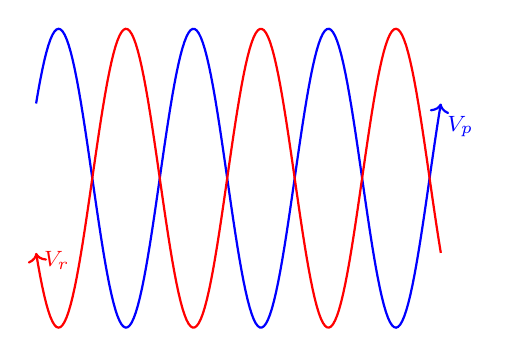
\begin{tikzpicture}
            \begin{axis}[
            axis x line=none,
            axis y line=none,
            ymax=1.5,
            ymin=-1.5,
            xmin=-pi,xmax=(pi*6)+(pi),
            x label style={anchor=north},,
            yticklabels={,,},
            xticklabels={,,},
            xtick=\empty,
            ytick=\empty,
            ]
            \addplot[domain=0:6*pi,samples=200,blue,thick,->]{cos(deg(x-pi/3))}
            node[right,pos=.99,font=\footnotesize]{$V_p$};
            \addplot[domain=0:6*pi,samples=200,red,thick,<-]{cos(deg(x-pi*1/3+pi))}
            node[left,pos=.1,font=\footnotesize]{$V_r$};
            \end{axis}
        \end{tikzpicture}        
    \end{center}
    \caption{Incident and reflected signal when $Z_L=0$}\label{fig:signal_with_Z_0}
\end{figure}
The voltage and the current over the line is:
\begin{equation}
    \begin{cases}
      V(l)&=V\bottomPlus\,e^{\,-j\beta l}-V\bottomMinus\,e^{\,j\beta l}=V\bottomPlus(e^{\,-j\beta l}+e^{\,j\beta l})=-2\,jV\bottomPlus\sin (\beta l)\\[5pt]
      I(l)&=\frac{V\bottomPlus}{Z_0}e^{\,-j\beta l}+\frac{V\bottomPlus}{Z_0}e^{\,j\beta l}=2\frac{V\bottomPlus}{Z_0}\cos (\beta l)
    \end{cases}
\end{equation}
So knowing only that $V\bottomPlus=-V\bottomMinus$ we can derive the voltage and current wave.\\
$\bullet$ If we go back in time domain:
\begin{align}
    \begin{split}
      V(l,t)&=\operatorname{Re}\left\{V(l)\,e^{\,j\omega t}\right\}=\operatorname{Re}\left\{j 2V\bottomPlus\sin (\beta l)\,e^{\,j\omega t}\right\}=\\[5pt]
      &=\operatorname{Re}\left\{j2V\bottomPlus\sin(\omega t)\,(\cos(\omega t)+j\sin(\omega t))\right\}=\\[5pt]
      &=-2\,|V\bottomPlus|\,\sin(\beta l)\sin(\omega t)
    \end{split}
\end{align}
Note that this is the equation of a \emph{stationary wave}! this mean that the voltage is moving across the line, but no information is transmitted from te generator to the load.\\
We can identify the stationary wave when $\beta l$ and $\omega t$ are in different $\cos$ (or $\sin$) operator.\\
$\bullet$ Power of this stationary wave:
\begin{align}
    \begin{split}
      P&=\frac{1}{2}V\cdot I^{*}=\frac{1}{2}\,\left(-2jV\bottomPlus \sin(\beta l)\right)\,\left(2\frac{V\bottomPlus}{Z_0}\cos(\beta l)\right)^*\\[5pt]
      &=-j2\frac{|V\bottomPlus|^2}{Z_0}\sin(\beta l)\cos(\beta l)
    \end{split}
\end{align}
Notice that the power is completely imaginary, this mean that we are transmitting only reactive power.\\
$\bullet$ The input impedance:
\begin{equation}\label{input_impedance_of_a_short}
    Z_i(l)=Z_0\frac{\cancelto{0}{Z_L}\cos(\beta l)+jZ_0 \sin(\beta l)}{Z_0\cos(\beta l)+j\cancelto{0}{Z_L}\sin(\beta l)}=jZ_0\tan(\beta l)
\end{equation}
$\bullet$ The input admittance:
\begin{equation}\label{input_admittance_of_an_open}
    Y_i(l)=\frac{1}{Z_i(l)}=\frac{1}{jZ_0\tan(\beta l)}=-Y_0\cot(\beta l)
\end{equation}
We again see that this input impedance is completely imaginary, so could be seen by the input port as a capacitor or an inductor depending on the sign of this imaginary number.\\
If we plot the behavior of $Z_i$ over $\frac{l}{\lambda}$ we have a graphical way to see this behavior (\cref{fig:behavior_of_short_in_TL}):
\begin{figure}[H]
    \begin{center}
        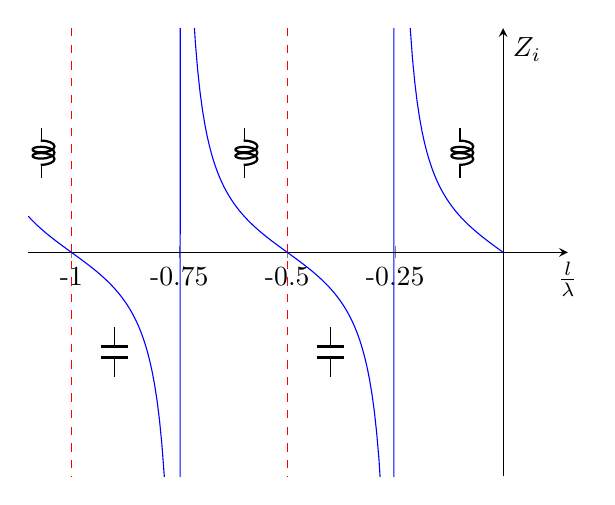
\begin{tikzpicture}
            \begin{axis}[
                axis x line=middle,
                axis y line=middle,
                xmin=-1.1,xmax=0.15,ymin=-4.5,ymax=4.5,
                x label style={anchor=north},
                xlabel= $\frac{l}{\lambda}$,
                ylabel={$Z_i$},
                yticklabels={,,},
                ytick=\empty,
                xticklabels={-1,-0.75,...,0},
                xtick={-1,-0.75,...,0},
                ]
              \addplot[domain=-1.1:0,blue,samples=200] {tan(deg(-x*2*3.14159))};
              \draw[dashed,red] (-1,-5) -- (-1,5);
              \draw[dashed,red] (-0.5,-5) -- (-0.5,5);

              \par\ctikzset{bipoles/capacitor/width=.1,bipoles/capacitor/height=.25}
              \draw (-0.9,-2.5) to [C] (-0.9,-1.5);
              \draw (-0.4,-2.5) to [C] (-0.4,-1.5);

              \par\ctikzset{bipoles/cuteinductor/width=.2,bipoles/cuteinductor/height=.25,bipoles/cuteinductor/coils=3}
              \draw (-0.6,2.5) to [cute inductor] (-0.6,1.5);
              \draw (-0.1,2.5) to [cute inductor] (-0.1,1.5);
              \draw (-1.07,2.5) to [cute inductor] (-1.07,1.5);
            \end{axis}
            
            \end{tikzpicture}       
    \end{center}
    \caption{Behavior of $Z_i$ a TL if the load is a short}\label{fig:behavior_of_short_in_TL}
\end{figure}
\subsubsection*{Another little exercise}
We have the usual information of our TL, but we know that the load is a short and on the behavior of the line is inductive; we need to find the length of the TL in order to have that behavior.\\
Data:
\begin{itemize}
    \item $v_p=2.07\cdot 10^{8}\si{\metre \per \second}$ speed of the signal.
    \item $L=15\si{\nano\henry}$ behavior of the TL.
    \item $f=3\si{\giga\hertz}$ frequency of the signal.
    \item $Z_0=50\si{\ohm}$ characteristic impedance of the TL.
\end{itemize}
Find length $l$.\\
$\bullet$ First of all we know that the load is a short, so:
\begin{equation*}
    Z_i(l)=jZ_0\, \tan(\beta l)
\end{equation*}
We also know that:
\begin{equation*}
    Z_i(l)=j\omega L
\end{equation*}
We go on to find the value of $l$:
\begin{align*}
    \begin{split}
      &Z_0\,\tan(\beta l)=\omega l\\[5pt]
      &\beta l=\arctan(\frac{\omega l}{Z_0})\\[5pt]
      &l=\frac{\lambda}{2\pi}\,\arctan(\frac{\omega l}{Z_0})=1.53\si{\metre}
    \end{split}
\end{align*}
This mean that if my TL described by the data i gave before measure $1.53\si{\metre}$, at the eye of the transmitter the TL is an inductor of $L=15\si{\nano\henry}$.\\
$\bullet$ If we change $f=4\si{\giga\hertz}$? Nothing to worry about:
\begin{equation*}
    \frac{l}{\lambda}=\frac{l\cdot f}{v_p}=0.3\geq 0.25
\end{equation*}
Assuming that \cref{fig:behavior_of_short_in_TL} is right, now the circuit should behave like a capacitor
Then we calculate $Z_i$:
\begin{equation*}
    Z_i=jZ_0\tan(\beta l)=jZ_0\tan(\frac{\omega}{v_p} l)=-j167.4
\end{equation*}
We obtained a negative imaginary impedance, so this is a capacitor!
\begin{equation*}
    -j\frac{1}{\omega C}=-j167.4 \rightarrow C=0.238\si{\pico\farad}
\end{equation*}
\subsection*{Transmission line wth an open circuit}
\begin{figure}[H]
    \begin{center}
        \begin{circuitikz} [ baseline=(current bounding box.center)]
            \ctikzset { label/align = straight }
            \draw (0,3)
            node[label={[font=\normalsize]above:$in$}] {}
            to[short, o-o,] (7,3)
            node[label={[font=\normalsize]above:$out$}] {}
            to[open](7.4,3)
            to[open={$Z_{l}=\infty$}] (7.4,0)
            to[open](7,0)
            to[short, o-o,] (0,0)
            ;
            \draw [-|] (0,-0.5) -- (7,-0.5)
            node[label={[font=\large]below:$0$}] {}
            ;
            \draw [->] (7,-0.5) -- (7.8,-0.5)
            node[label={[font=\large]right:$l$}] {}
            ;
            \draw (4,1)node[label={[font=\LARGE]above:$Z_0$}] {}
            ;
          \end{circuitikz}     
    \end{center} \caption{Transmission line with open circuit load}\label{fig:transmission_line_open}
  \end{figure}
In this case we do the opposite as before, we put an open circuit at the output of the TL, in this case $Z_L=\infty$.\\
Instead to have the voltage equal to 0 at the load, we have the current equal to zero:
\begin{equation}
    I(l)=\frac{V\bottomPlus}{Z_0}\,e^{\,-j\omega l}-\frac{V\bottomMinus}{Z_0}\,e^{\,-j\omega l}
\end{equation}
\begin{equation}
    I(l=0)=I_L=0=I\bottomPlus+I\bottomMinus = \frac{1}{Z_0}\,\left[V\bottomPlus-V\bottomMinus\right] \;\rightarrow \;V\bottomPlus=V\bottomMinus
\end{equation}
$\bullet$ For the reflection coefficient this mean:
\begin{equation}
    \rho_L=\frac{V\bottomMinus}{V\bottomPlus}=\frac{V\bottomPlus}{V\bottomPlus}=1
\end{equation}
And this mean that:
\begin{center}
    \begin{tabular}{ c c c }
        $|\rho_L|=1$&
        and&
        $\phase{\rho_L}=0^{\circ}$
    \end{tabular}
\end{center}
$\bullet$ We do the same calculation we already with the open circuit, then wu obtain the voltage and the current over the line:
\begin{equation}
    \begin{cases}
      V(l)&=V\bottomPlus\,e^{\,-j\beta l}-V\bottomMinus\,e^{\,j\beta l}=V\bottomPlus(e^{\,-j\beta l}-e^{\,j\beta l})=2\,jV\bottomPlus\sin (\beta l)\\[5pt]
      I(l)&=\frac{V\bottomPlus}{Z_0}e^{\,-j\beta l}-\frac{V\bottomPlus}{Z_0}e^{\,j\beta l}=-2\frac{V\bottomPlus}{Z_0}\cos (\beta l)
    \end{cases}
\end{equation}
Again if we go back to time domain we will notice that we are looking at a stationary wave.\\
$\bullet$ The calculation for the input impedance is a bit different, but at the end we obtain:
\begin{equation}\label{eq:open_circuit_TL}
    Z_i(l)=\lim_{Z_0\rightarrow\infty} Z_0\frac{Z_L\cos(\beta l)+jZ_0 \sin(\beta l)}{Z_0\cos(\beta l)+jZ_L\sin(\beta l)}=jZ_0\cot(\beta l)
\end{equation}
$\bullet$ The input admittance:
\begin{equation}\label{input_admittance_of_a_short}
    Y_i(l)=\frac{1}{Z_i(l)}=\frac{1}{jZ_0\cot(\beta l)}=-Y_0\tan(\beta l)
\end{equation}
$\bullet$ We can plot again the behavior of the TL, that is very similar as before, but mirrored at the $x$ axe:
\begin{figure}[H]
    \begin{center}
        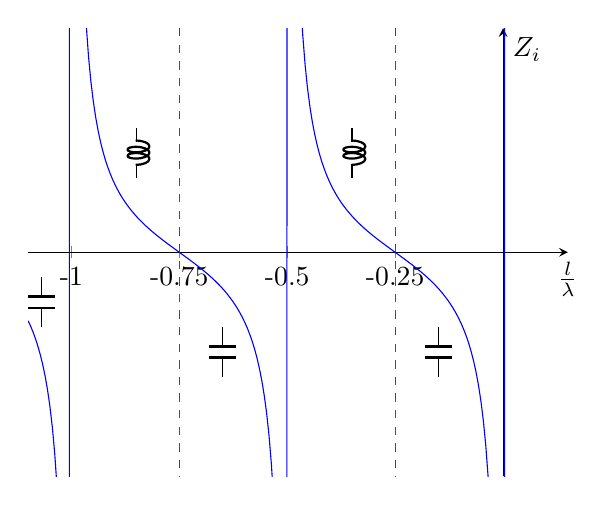
\begin{tikzpicture}
            \begin{axis}[
                axis x line=middle,
                axis y line=middle,
                xmin=-1.1,xmax=0.15,ymin=-4.5,ymax=4.5,
                x label style={anchor=north},
                xlabel= $\frac{l}{\lambda}$,
                ylabel={$Z_i$},
                yticklabels={,,},
                ytick=\empty,
                xticklabels={-1,-0.75,...,0},
                xtick={-1,-0.75,...,0},
                ]
              \addplot[domain=-1.1:0.01,blue,samples=200] {-cot(deg(-x*2*3.14159))};
              \draw[dashed,red] (-0.75,-5) -- (-0.75,5);
              \draw[dashed,red] (-0.25,-5) -- (-0.25,5);

              \par\ctikzset{bipoles/capacitor/width=.1,bipoles/capacitor/height=.25}
              \par\ctikzset{bipoles/cuteinductor/width=.2,bipoles/cuteinductor/height=.25,bipoles/cuteinductor/coils=3}

              \draw (-0.85,2.5) to [cute inductor] (-0.85,1.5);
              \draw (-0.35,2.5) to [cute inductor] (-0.35,1.5);

              \draw (-0.65,-2.5) to [C] (-0.65,-1.5);
              \draw (-0.15,-2.5) to [C] (-0.15,-1.5);
              \draw (-1.07,-1.5) to [C] (-1.07,-0.5);
            \end{axis}
            
            \end{tikzpicture}       
    \end{center}
    \caption{Behavior of $Z_i$ a TL if the load is an open}\label{fig:behavior_of_open_in_TL}
\end{figure}
\subsection*{Last little curiosity if the signal is an EMF}
Until now we have seen a signal over a TL, but can we consider all those thing in the free space with the EMF? It depend, let's see how:
\subsubsection*{Short circuit in EMF}
It is possible to use a metallic conductor material at the output to impose the electric field on the surface equal to zero. It is like to send the EMF to a wall made of metal.
\subsubsection*{Open circuit in EMF}
As we have done before, we should send the EMF to a wall made by a material that let the magnetic material equal to zero... but this does not exist, or at least we didn't find it yet.
\section{Class 6 - 15/03/21}
\subsection*{Transmission line with general load $\bm{Z_0}$}
In the previous lectures we saw the transmission line in short circuit or open circuit, but those case are not the most common one, today we will see the most general situation when the load is a complex number $Z_L=a+jb$, like in \cref{fig:tl_with_general_load}.
\begin{figure}[H]
    \begin{center}
        \begin{circuitikz} 
            \draw (2,2)
            to[short, o-o] (7,2)
            to[short] (8.5,2)
            to[generic=$Z_{l}$] (8.5,0)
            to[short, -o](7,0)
            to[short, -o](2,0)
            ;
            \draw (4.5,0.45)node[label={[font=\LARGE]above:$Z_0$}] {}
            ;
          \end{circuitikz}     
    \end{center} \caption{Forward and backward wave signal in a TL}\label{fig:tl_with_general_load} 
\end{figure}
%We recall the voltage wave equation: $V\bottomPlus\,e^{\,j\beta l}+V\bottomMinus\,e^{\,-j\beta l}$.\\
% What we want for a great TL is to have only $V\bottomPlus$, or at least $V\bottomPlus > V\bottomMinus$
Now, what we want to do is to attempt some magic trick to modify the wave equation in \cref{eq:wave_solution_no_losses}, maybe we find a way to evaluate better how the reflected signal is affecting the line.
\begin{equation}
    V\bottomPlus =(V\bottomPlus - V\bottomMinus) + V\bottomMinus
\end{equation}
Then we can write the voltage over the line as:
\begin{align}
    \begin{split}
      V(l)&=\left[(V\bottomPlus - V\bottomMinus)+V\bottomMinus\right]e^{\,-j\beta l}+V\bottomMinus\,e^{\,j\beta l}=\\[5pt]
      &=(V\bottomPlus - V\bottomMinus)e^{\,j\beta l}+V\bottomMinus\,e^{\,-j\beta l}+V\bottomMinus\,e^{\,j\beta l}=\\[5pt]
      &=(V\bottomPlus - V\bottomMinus)e^{\,j\beta l}+V\bottomMinus\,\left(e^{\,-j\beta l}+e^{\,j\beta l}\right)=\\[5pt]
      &=(V\bottomPlus - V\bottomMinus)e^{\,j\beta l}+2\,V\bottomMinus\,\cos(\beta l)
    \end{split}\label{eq:new_form_of_voltage_over_TL}
  \end{align}
  We skipped some passages, but that should only be the application of the trigonometric form of a complex number.\\
  We can notice from \cref{eq:new_form_of_voltage_over_TL} that the voltage over a TL is composed by two terms:
  \begin{itemize}
      \item $\bm{(V\bottomPlus - V\bottomMinus)e^{\,j\beta l}}$: This is the equation of a direct wave with amplitude $(V\bottomPlus - V\bottomMinus)$. The amplitude is not $V\bottomPlus$ because part of the wave is reflected backward
      \item $\bm{2\,V\bottomMinus\,\cos(\beta l)}$: This is the expression of a stationary wave. This part is "eating" part of the forward wave, this mean that if i fall in some "unlucky" point inside my TL the signal will be distorted.
  \end{itemize}

If i want to go back to the time domain with the forward wave using the usual formula in \cref{eq:from_phas_to_time_TL}:
\begin{equation}
    V(l,t)=(V\bottomPlus - V\bottomMinus)\cos(\omega t-\beta l)+2V\bottomMinus\cos(\omega t)\cos(\beta l)
\end{equation}
We find again a stationary wave (just as expected).
\subsection*{Module of the voltage wave in phasor}
Before to introduce the next topic (SWR), we need to introduce how we can calculate the module of the voltage wave in phasor domain.\\
In \cref{fig:voltage_components_in_phas} you can see the graphical representation of the two components that build up the voltage wave in complex domain that we have already seen in \cref{eq:current_and_voltage_in_TL_phas}.
\begin{figure}[H]    
    \begin{center}
        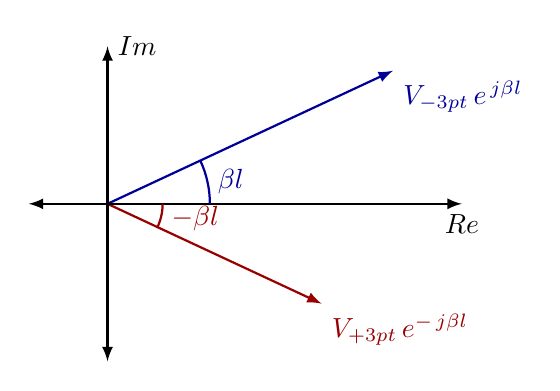
\begin{tikzpicture}[>=latex]
            \draw[style=help lines] (0,0) (3,2);
        
            \coordinate (vec1) at (-25:3); 
            \coordinate (vec2) at (25:4);
            \coordinate (vec3) at (0:4.5);
            \coordinate (vec4) at (90:2);
            \coordinate (vec5) at (270:2);
            \coordinate (vec6) at (180:1);
        
            \draw[->,thick,blue!60!black] (0,0) -- (vec2) node[below right] {$V\bottomMinus\,e^{\,j\beta l}$}; 
            \draw[->,thick,red!60!black] (0,0) -- (vec1) node[below right] {$V\bottomPlus\,e^{-\,j\beta l}$};
            \draw[->,thick,black] (0,0) -- (vec3) node [below] {$Re$};
            \draw[->,thick,black] (0,0) -- (vec4) node [right] {$Im$};
            \draw[->,thick,black] (0,0) -- (vec5);
            \draw[->,thick,black] (0,0) -- (vec6);
        
            \draw [blue!60!black, thick] (1.3,0) 
            arc [start angle=0, end angle=25, radius=1.3cm]
            node [midway, right] {$\beta l$}; 
            \draw [red!60!black, thick] (0:0.7) 
            arc [start angle=0, end angle=-26, radius=0.7cm]
                node [midway, right,yshift=-1] {$-\beta l$};
        \end{tikzpicture}
    \end{center}\caption{Forward and backward Voltage wave in phasor domain}\label{fig:voltage_components_in_phas}
\end{figure}
What we are doing now is to find a proper way to describe the module of $\phas{V}(l)$, that is NOT the real voltage value in the TL (remember that we are in phasor domain).\\
If you remember how we defined $\rho$\footnote{remember that $\rho$ and $\rho_L$ are the same thing with different name} in \cref{eq:reflection_coeff_at_load}, there is no doubt that we can write:
\begin{equation*}
    \rho= \frac{V\bottomMinus}{V\bottomPlus}
\end{equation*}
So the voltage equation in \cref{fig:voltage_components_in_phas} will become:
\begin{align}
    \begin{split}
        \phas{V}(l) &= V\bottomPlus \,e^{\,-j\beta l}+\rho\, V\bottomPlus \,e^{\,j\beta l}=\\[5pt]
        &= V\bottomPlus \left(e^{\,-j\beta l}+\rho \, e^{\,j\beta l}\right)
    \end{split}
\end{align}
Now, the best way to compute the module is to obtain it from $|\phas{V}(l)|^2$:
\begin{align}
    \begin{split}
        |\phas{V}(l)|^2 &= \phas{V}(l)\,\phas{V}^*(l) =\\[5pt]
        &=|V\bottomPlus|^2\,\left(e^{\,-j\beta l}+\rho \, e^{\,j\beta l}\right)\,\left(e^{\,-j\beta l}+\rho \, e^{\,j\beta l}\right)^*=\\[5pt]
        &= |V\bottomPlus|^2\,\left(e^{\,-j\beta l}+\rho \, e^{\,j\beta l}\right)\,\left(e^{\,j\beta l}+\rho^* \, e^{\,-j\beta l}\right)=\\[5pt]
        &=|V\bottomPlus|^2\,\left(1+|\rho|^2+\rho\,e^{\,j2\beta l}+\rho^* \, e^{\,-j2\beta l}\right)
    \end{split}
\end{align}
Let's assume $\varphi $ is the phase of the complex number $\rho=|\rho|e^{\,j\varphi}$:
\begin{align}
    \begin{split}
        |\phas{V}(l)|^2 &=|V\bottomPlus|^2\,\left(1+|\rho|^2+|\rho|\,e^{\,j(2\beta l+\varphi)}+|\rho| \, e^{\,-j(2\beta l+\varphi)}\right)=\\[5pt]
        &=|V\bottomPlus|^2\,\left(1+|\rho|^2+|\rho|\left[e^{\,j(2\beta l+\varphi)}+ e^{\,-j(2\beta l+\varphi)}\right]\right)=\\[5pt]
        &=|V\bottomPlus|^2\,\left[  1+|\rho|^2+|\rho|\cos(2\beta l+\varphi)  \right]
    \end{split}
\end{align}
From here we can easily obtain the expression for $|\phas{V}(l)|=\sqrt{|\phas{V}(l)|^2}$ and also for $|\phas{I}(l)|$ (the calculation are very similar):
\begin{equation}
    \begin{cases}
        |\phas{V}(l)| =|V\bottomPlus|\sqrt{1+|\rho|^2+|\rho|\cos(2\beta l+\varphi)}\\
        |\phas{I}(l)| =\frac{|V\bottomPlus|}{Z_0}\sqrt{1+|\rho|^2-|\rho|\cos(2\beta l+\varphi)}
    \end{cases}\label{eq:module_of_v_and_i}
\end{equation}
From what we can see in \cref{eq:module_of_v_and_i}, the module of both voltage and current in phasor domain increase and decrease periodically along $l$ because $\cos \in [-1,1]$
\subsubsection*{Obtaining $\bm{V_{max}}$ and $\bm{V_{min}}$}
We have already seen the refraction ratio $\rho$, but we can introduce a better parameter to describe how distorted is my signal. To do so we need to have a closer look at the module of the voltage in phasor domain that we have seen in the last section.\\
As we said, the $\cos$ inside the expression of $|\phas{V}(l)|$ is periodic thanks to the $\cos$ inside it, so we can know the maximum and minimum value of $|\phas{V}(l)|$ and $|\phas{I}(l)|$ moving along $l$.\\
From \cref{eq:module_of_v_and_i} we can simply find those values by replacing $\cos$ with respectively $+1$ and $-1$:

\begin{equation}
    \begin{cases}
        V_{max} =|V\bottomPlus|\sqrt{1+|\rho|^2+2|\rho|}=|V\bottomPlus|(1+|\rho|)\\
        V_{min} =|V\bottomPlus|\sqrt{1+|\rho|^2-2|\rho|}=|V\bottomPlus|(1-|\rho|)
    \end{cases}\label{eq:vmin_e_vmax}
\end{equation}
From here, we assume that we have found a certain $l_0$ value where we can find the maximum value of $|V(l_0)|$:
\begin{align}
    \begin{split}
    |V(l_0)|&=|V\bottomPlus|(1+|\rho|)=\\[5pt]
    &=|V\bottomPlus|+|V\bottomMinus|=V_{max}\\[5pt]
    \end{split}
\end{align}
If i move from that section of the line, the phase will not be equal anymore and we will not see $V_{max}$ anymore.\\
Just a little example if i move by $\Delta L=\frac{\lambda}{4}$ from $V_{max}$, we will reach the minimum:
\begin{align}
    \begin{split}
        \left|V\left(l_0+\frac{\lambda}{4}\right)\right|&=|V\bottomPlus|(1-|\rho|)=\\[5pt]
        &=|V\bottomPlus|-|V\bottomMinus|=V_{min}\\[5pt]
    \end{split}\label{eq:v_minimum}
\end{align}
Why this? Look at \cref{eq:module_of_v_and_i}, here you can see that to reach $\cos(\cdots)=-1$ we need to move its argument from $0$ to $\pi$, and $\frac{\lambda}{4}$ fits this purpose:
\begin{align}
    \begin{split}
        &\left(2\beta \left(l_0+\frac{\lambda}{4}\right) +\varphi\right) = \\[5pt]
        &=\left(\cancelto{0}{2\beta l_0 +\varphi} +2\beta \frac{\lambda}{4}\right)\\[5pt]
        &=\left(2\,\frac{2\pi}{\lambda} \frac{\lambda}{4} \right)=(\pi)\\[5pt]
    \end{split}
\end{align}
A little recap:
\begin{equation}
    \begin{cases}
        V_{max} =(|V\bottomPlus|+|V\bottomMinus|)\\
        V_{min} =(|V\bottomPlus|-|V\bottomMinus|)
    \end{cases}
\end{equation}
As we can see in \cref{eq:v_minimum}, we reached the minimum value $V_{min}$ by moving from $V_{max}$ by $\Delta L=\frac{\lambda}{4}$, so it was not just a little example but it is very important!\\
Again if i move by another $\Delta L=\frac{\lambda}{4}$ from $V_{min}$ we reach another maximum and so on \dots
\begin{figure}[H]
    \begin{center}
        \begin{circuitikz} [ baseline=(current bounding box.center)]
            \ctikzset { label/align = straight }
            \draw [-|] (1,-0.5) -- (2,-0.5)
            node[label={[font=\large]above:$V_{min}$}] {}
            ;
            \draw [-|] (2,-0.5) -- (4,-0.5)
            node[label={[font=\large]above:$V_{max}$}] {}
            node[midway,yshift=-1em]{$\frac{\lambda}{4}$};;
            \draw [-|] (4,-0.5) -- (6,-0.5)
            node[label={[font=\large]above:$V_{min}$}] {}
            node[midway,yshift=-1em]{$\frac{\lambda}{4}$};;
            \draw [-|] (6,-0.5) -- (8,-0.5)
            node[label={[font=\large]above:$V_{max}$}] {}
            node[label={[font=\large]below:$0$}] {}
            node[midway,yshift=-1em]{$\frac{\lambda}{4}$};
            ;
            \draw [->] (8,-0.5) -- (8.8,-0.5)
            node[label={[font=\large]right:$l$}] {}
            ;
          \end{circuitikz}     
    \end{center} \caption{Voltage behavior over the line}
\end{figure}
\subsubsection*{Obtaining $\bm{I_{max}}$ and $\bm{I_{min}}$}
Obviously, everything that we said until now can be said also for the current.\\
Starting from \cref{eq:module_of_v_and_i} we can again replace the $\cos$ with $-1$ and $+1$ and obtain the maximum and minimum value of $|\phas{I}(l)|$
\begin{equation}
    \begin{cases}
        I_{max} =\frac{|V\bottomPlus|}{Z_0}\sqrt{1+|\rho|^2-2|\rho|}=\frac{|V\bottomPlus|}{Z_0}(1-|\rho|)\\
        I_{min} =\frac{|V\bottomPlus|}{Z_0}\sqrt{1+|\rho|^2+2|\rho|}=\frac{|V\bottomPlus|}{Z_0}(1+|\rho|)
    \end{cases}\label{eq:imin_e_imax}
\end{equation}
The real differences between the voltage and current equation are $\frac{1}{Z_0}$ and the fact that the minus is swapped.\\
If we do the same calculation that we have done for the voltage we can obtain:
\begin{equation}
    \begin{cases}
        I_{max} =(|I\bottomPlus|+|I\bottomMinus|)\\
        I_{min} =(|I\bottomPlus|-|I\bottomMinus|)
    \end{cases}
\end{equation}
We can notice that the periodic behavior remains the same, but $I_{max}$ is shifted from $V_{max}$ by $\frac{\lambda}{4}$, this also mean that $I_{max}$ and $V_{min}$ share the same position on the line:
\begin{figure}[H]
    \begin{center}
        \begin{circuitikz} [ baseline=(current bounding box.center)]
            \ctikzset { label/align = straight }
            \draw [-|] (1,-0.5) -- (2,-0.5)
            node[label={[font=\large]above:$V_{min}$}] {}
            node[label={[font=\large]above:$I_{max}$},yshift=1.5em] {}
            ;
            \draw [-|] (2,-0.5) -- (4,-0.5)
            node[label={[font=\large]above:$V_{max}$}] {}
            node[label={[font=\large]above:$I_{min}$},yshift=1.5em] {}
            node[midway,yshift=-1em]{$\frac{\lambda}{4}$};
            \draw [-|] (4,-0.5) -- (6,-0.5)
            node[label={[font=\large]above:$V_{min}$}] {}
            node[label={[font=\large]above:$I_{max}$},yshift=1.5em] {}
            node[midway,yshift=-1em]{$\frac{\lambda}{4}$};
            \draw [-|] (6,-0.5) -- (8,-0.5)
            node[label={[font=\large]above:$V_{max}$}] {}
            node[label={[font=\large]above:$I_{min}$},yshift=1.5em] {}
            node[label={[font=\large]below:$0$}] {}
            node[midway,yshift=-1em]{$\frac{\lambda}{4}$};
            ;
            \draw [->] (8,-0.5) -- (8.8,-0.5)
            node[label={[font=\large]right:$l$}] {}
            ;
          \end{circuitikz}     
    \end{center} \caption{Voltage behavior over the line}
\end{figure}
\subsubsection*{Obtaining $\bm{Z_{max}}$ and $\bm{Z_{min}}$}
With that being said, we can also introduce the maximum and minimum\\
impedance:
\begin{equation}
    \begin{cases}
        Z_{max} = \frac{V_{max}}{I_{max}}\\
        Z_{min} = \frac{V_{min}}{I_{min}}
    \end{cases}
\end{equation}
And:
\begin{equation}
    Z_{max}=\frac{V_{max}}{I_{max}}=\frac{|V\bottomPlus|+|V\bottomMinus|}{|V\bottomPlus|-|V\bottomMinus|}\,Z_0
\end{equation}
\subsection*{Standing wave ratio (SWR)}
Finally we can introduce this famous value of Standing wave ratio (SWR). This is very useful to describe the quality of our signal when we have a forward and backward wave.
\begin{equation}
    \text{SWR}=\frac{V_{max}}{V_{min}}=\frac{1+|\rho|}{1-|\rho|}
\end{equation}
Another interesting relation is the one with the maximum and minimum\\
impedance.\\
For $Z_{max}$:
\begin{equation}
    \begin{cases}
        Z_{max} = \text{SWR}\,Z_0 \\
        Z_{min} = \frac{Z_0}{\text{SWR}}
    \end{cases}
\end{equation}
We can also refer to those values as normalized to $Z_0$, this will help a bit the calculations during exercises.
\begin{equation}
    \begin{cases}\label{eq:normalized_impedance}
        \mathcal{Z}_{max} = \frac{Z_{max}}{Z_0}=\text{SWR}\\
        \mathcal{Z}_{min} = \frac{Z_{min}}{Z_0}=\frac{1}{\text{SWR}}
    \end{cases}
\end{equation}
This last part is a bit different from what explained the prof during lectures, but i think that during this class he was not very clear with math, so i decided to consult the world wide web, and i've actually found a really interesting free book available at \cite{Ellingson2020Book}.
\subsection*{Little exercise \#1}
Now we will do some simple exercise useful to better comprehend what we are saying.\\
In the first exercise we have a transmission line in  where we need to find the SWR.
\begin{figure}[H]
    \begin{center}
        \begin{circuitikz} 
            \draw (2,2)
            to[short, o-o] (7,2)
            to[short] (8.5,2)
            to[generic={$Z_{l}=?$}] (8.5,0)
            to[short, -o](7,0)
            to[short, -o](2,0)
            ;
            \draw (4.5,0.45)node[label={[font=\Large]above:$Z_0=50\si{\ohm}$}] {}
            ;
            \draw [-]  (2.5,2.5) -- (2.5,-0.5)
            node[label={right:{$Z_i=(50+j150) \si{\ohm}$}}] {}
            ;
            \draw [->]  (2.5,1) -- (2.8,1)
            ;
          \end{circuitikz}     
    \end{center} \caption{Transmission line of exercise 2}\label{fig:exercise_1_class6} 
\end{figure}
First of all we normalize the input impedance 
\begin{equation*}
    \mathcal{Z}_i=\frac{Z_i}{Z_0}=(1-j3)
\end{equation*}
Then we need the reflection coefficient on the load:
\begin{equation*}
    \rho_L=\frac{Z_i-Z_0}{Z_i+Z_0}=\frac{\mathcal{Z}_i - 1}{\mathcal{Z}_i + 1}=\frac{1-j3-1}{1-j3+1}=0.7-j0.46
\end{equation*}
Note that we didn't specified the position $l$ because the data already give us the value of the input impedance.\\
The module of the reflection coefficient is: $|\rho(l)|=0.83$
Now it is very simple to obtain the SWR:
\begin{equation*}
    \text{SWR}=\frac{1+|\rho|}{1-|\rho|}=\frac{1+0.83}{1-0.83}=10.76
\end{equation*}
The SWR value is higher than 10, and it is not a very good value :/
\subsection*{Little exercise \#2}
In this second exercise we have a UHF antenna in an airplane (don't ask me why all those strange details) working in a range of frequency $f=225-400\si{\mega\hertz}$.\\
Now, inside the airplane there is a transmission line with $Z_0=50\si{\ohm}$ where signal is transmitted from the cabinet to the antenna. We know that for different frequencies the antenna behave like a different load $Z_L$:
\begin{center}
    \begin{tabular}{|c|c|}
        \hline
        frequency&input impedance $Z_L$\\
        \hline
        $225$\si{\mega\hertz}&$22.5-j51$ \si{\ohm}\\
        \hline
        $300$\si{\mega\hertz}&$35-j16$ \si{\ohm}\\
        \hline
        $400$\si{\mega\hertz}&$45-j2.5$ \si{\ohm} \\
        \hline
    \end{tabular}
\end{center}
Now we need to find $\rho_L$ and SWR.\\
First of all we use the normalized impedance so simplify things:
\begin{equation*}
    \mathcal{Z}_L=\frac{Z_L}{Z_0}
\end{equation*}
Then it is very simple to obtain $\rho_L$:
\begin{equation*}
    \rho_L=\frac{\mathcal{Z}_L-1}{\mathcal{Z}_L+1}
\end{equation*}
As we have done before, we can calculate the module of $\rho$ then the SWR is:
\begin{equation*}
    \text{SWR}=\frac{1+|\rho|}{1-|\rho|}
\end{equation*}
\subsection*{Little exercise \#3}
We consider a transmission line with a length of $75\si{\centi\metre}$
\begin{figure}[H]
    \begin{center}
        \begin{circuitikz} 
            \draw (2,2)
            to[short, o-o] (7,2)
            to[short] (8.5,2)
            to[generic={$Z_{l}=140\si{\ohm}$}] (8.5,0)
            to[short, -o](7,0)
            to[short, -o](2,0)
            ;
            \draw (4.5,0.45)node[label={[font=\Large]above:$Z_0=70\si{\ohm}$}] {}
            ;
            \draw [->]  (2.5,2.3) -- (6.5,2.3)
            node[midway,yshift=0.6em]{$75\si{\centi\metre}$};;
          \end{circuitikz}     
    \end{center} \caption{Transmission line of exercise 3}\label{fig:exercise_3_class6} 
\end{figure}
In this transmission line we can have signals with different frequencies:
\begin{center}
    \begin{tabular}{|c|}
        \hline
        frequency\\
        \hline
        $50\si{\mega\hertz}$\\
        \hline
        $100\si{\mega\hertz}$\\
        \hline
        $150\si{\mega\hertz}$\\
        \hline
        $200\si{\mega\hertz}$\\
        \hline
    \end{tabular}
\end{center}
We want to calculate the input impedance $Z_i$. We just remind that 
\begin{equation*}
    \beta l=\frac{2\pi}{\lambda}=\frac{2\pi}{c}\,fl
\end{equation*}
We calculate $\beta$ for each frequencies, then we can calculate $Z_i$:
\begin{equation*}
    Z_i=Z_0\frac{Z_L\,\cos(\beta l)+jZ_0\sin(\beta l)}{Z_0\,\cos(\beta l)+jZ_L\sin(\beta l)}
\end{equation*}
I won't do all the calculations here, but the results are:
\begin{itemize}
    \item $\bm{f=50}\si{\mega\hertz}\bm{\rightarrow Z_i=56-j42}\si{\ohm}$.
    \item $\bm{f=100}\si{\mega\hertz}\bm{\rightarrow Z_i=35}\si{\ohm}$: That is very interesting!\\
    Note that $l=0.75\si{\metre}$ and $\lambda=3\si{\metre}$, and $l=\frac{\lambda}{4}$ so we have reached a minimum or a maximum.\\
    We know that this is a minimum because we are at $l=\frac{\lambda}{4}$ from $l=0$ where we have the actual impedance.\\
    If we calculate the normalized impedance for the maximum and minimum value: $\mathcal{Z}_{min}=\frac{140}{70}=2$ and $\mathcal{Z}_{min}=\frac{35}{70}=\frac{1}{2}$.\\
    Then we notice that $\mathcal{Z}_{min}=\frac{1}{\mathcal{Z}_{max}}$
    \item $\bm{f=150}\si{\mega\hertz}\bm{\rightarrow Z_i=56+j42}\si{\ohm}$.
    \item \item $\bm{f=200}\si{\mega\hertz}\bm{\rightarrow Z_i=140}\si{\ohm}$: This is $Z_{max}$
\end{itemize}
\subsection*{Smith chart}
All those numbers and complex numbers are quite confusing... But what if i tell you that there is a graphical way to describe the transmission line and all the useful coefficient.\\
We need to prepare ourself a bit, first of all we need to define a bit better the normalized impedance (already seen in \cref{eq:normalized_impedance}):
\begin{equation}
    \mathcal{Z}_i(l)=\frac{Z_i(l)}{Z_0}=\mathcal{R}+j\mathcal{X}
\end{equation}
We also remember the reflection coefficient $\rho$:
\begin{equation}
    \rho(l)=\rho_L e^{\,j2\beta l}=u+jv
\end{equation}
Those two parameters are dependent on $l$, but now we consider that we have chosen a $l*$ value so $\mathcal{Z}$ and $\rho$ are fixed.\\
Consider the input impedance for a given position on the TL and we can now write:
\begin{align}
    \begin{split}
        \mathcal{Z}_i(l^*) &=\frac{Z_{in}}{Z_0}\\[5pt]
        &=\frac{1}{Z_0}\cdot \frac{V(l^*)}{I(l^*)}\\[5pt]
        &=\frac{1}{\cancel{Z_0}}\cdot \cancel{Z_0} \,\frac{V\bottomPlus +V\bottomMinus }{V\bottomPlus -V\bottomMinus }\\[5pt]
        &= \frac{V\bottomPlus +\rho V\bottomPlus }{V\bottomPlus -\rho V\bottomPlus } = \frac{1 +\rho }{1 -\rho }
    \end{split}
\end{align}
We simplify a bit the notation and we continue:
\begin{align}
    \begin{split}
        \mathcal{Z}_i =\frac{1+\rho}{1-\rho}& =\frac{1+u+jv}{1-u-jv}\cdot \frac{1-u+jv}{ 1-u+jv}=\mathcal{R}+j\mathcal{X}\\[5pt]
        \mathcal{R}+j\mathcal{X}&=\frac{(1-u^2-v^2)+j2v}{(1-u)^2+v^2}
    \end{split}
\end{align}
Then if we split the real from the imaginary part:
\begin{center}
    \begin{tabular}{ c c c }
        $\mathcal{R}=\frac{1-(u^2+v^2)}{(1-u)^2+v^2}$&
        &
        $\mathcal{X}=\frac{2v}{1-u^2+v^2}$
    \end{tabular}
\end{center}
We do some more calcultations with $\mathcal{R}$:
\begin{align}
    \begin{split}
        &[(1-u)^2+v^2]\,\mathcal{R}=1-(u^2+v^2)\\[5pt]
        &\mathcal{R}\, u^2 -2 u\, \mathcal{R} + \mathcal{R} + \mathcal{R} v^2 +u^2+v^2=1\\[5pt]
        &(1+\mathcal{R})u^2-2u\,\mathcal{R}+\mathcal{R}+(1+\mathcal{R})v^2=1\\[5pt]
        &u^2-2\frac{\mathcal{R}}{1+\mathcal{R}}u+\frac{\mathcal{R}}{1+\mathcal{R}}+v^2=\frac{1}{1+\mathcal{R}}
    \end{split}
\end{align}
Then we add on left and on right the same number: $\left(\frac{\mathcal{R}}{1+\mathcal{R}}\right)^2$\\
And we can write:
\begin{equation}
    \left(u-\frac{\mathcal{R}}{1+\mathcal{R}}\right)^2+v^2=\frac{1}{1+\mathcal{R}} - \frac{\mathcal{R}}{1+\mathcal{R}}+\left(\frac{\mathcal{R}}{1+\mathcal{R}}\right)^2
\end{equation}
Some math passage later that we will not show\dots
\begin{equation}
    \begin{cases}
        \left(u-\frac{\mathcal{R}}{1+\mathcal{R}}\right)^2+v^2 =\frac{1}{(1+\mathcal{R})^2}\\
        (u-1)^2+\left(v-\frac{1}{\mathcal{X}}\right)^2=\frac{1}{\mathcal{X}^2}
    \end{cases}
\end{equation}
FINALLY, so what is happening here?\\
We notice that the first equation is the equation of a circle centered in $\left(\frac{\mathcal{R}}{1+\mathcal{R}},0\right)$ and radius $\frac{1}{\mathcal{R}+1}$.\\
In \cref{fig:x_cicles} you can see some plots of this circle with different value of $\mathcal{R}$
\begin{figure}[H]
\begin{center}
    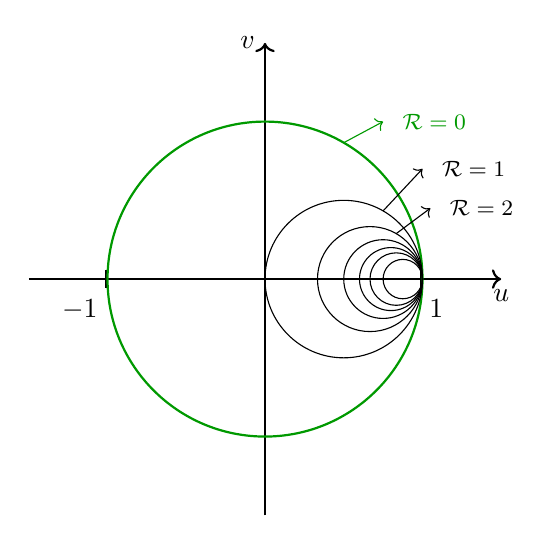
\begin{tikzpicture}
        % Axis
        \draw [thick,-|,black] (-3,0) -- (-2,0)
            node[label={below:$-1$},xshift=-1em] {};
            \draw [thick,-|,black] (-2,0) -- (2,0)
            node[label={below:$1$},xshift=0.5em] {};
        \draw[thick,->,black] (2,0)--(3,0) node[below] {$u$}; % x axis
        \draw[thick,->,black] (0,-3)--(0,3) node[left] {$v$}; % y axis
        \draw[green!60!black,thick] (0,0) circle (2);
        \draw[->,green!60!black] (1,1.732)--(1.5,2)
        node[label={[font=\footnotesize]right:$\mathcal{R}=0$}] {};
        \draw[black] (1,0) circle (1);
        \draw[->,black] (1.5,0.866)--(2,1.4)
        node[label={[font=\footnotesize]right:$\mathcal{R}=1$}] {};
        \draw[black] (4/3,0) circle (2/3);
        \draw[->,black] (2*5/6,0.866*2/3)--(2.1,0.9)
        node[label={[font=\footnotesize]right:$\mathcal{R}=2$}] {};
        \draw[black] (3*2/4,0) circle (2/4);
        \draw[black] (4*2/5,0) circle (2/5);
        \draw[black] (5*2/6,0) circle (2/6);
        \draw[black] (7*2/8,0) circle (2/8);
       \end{tikzpicture}
\end{center}\caption{Plots of different circles from the first equation}\label{fig:x_cicles} 
\end{figure}
All the circumference will collapse in $(1,0)$ when $\mathcal{R}\rightarrow\infty$\\.
For $\mathcal{R}=0$ we find the limit circumference (green one in \cref{fig:x_cicles}), this is the limit because we can not have negative real impedance.\\
Good news for the second equation in \cref{eq:normalized_impedance}, because also with this we can find some circumferences with center in $(1,\frac{1}{\mathcal{X}})$ and radius $\frac{1}{\mathcal{X}}$:
\begin{figure}[H]
    \begin{center}
        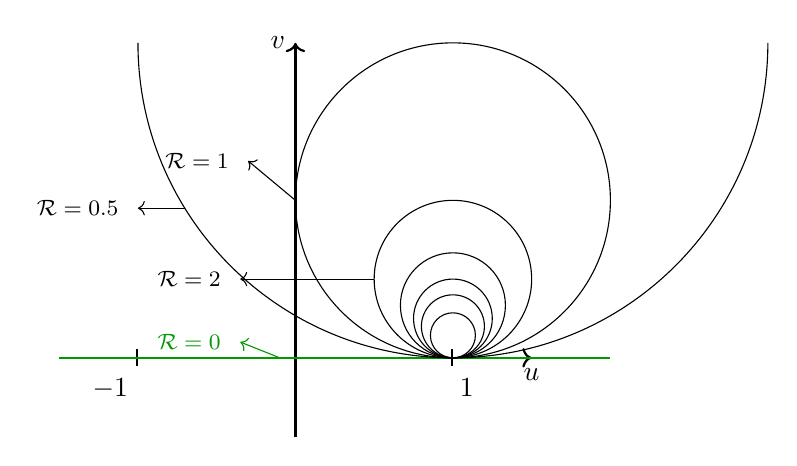
\begin{tikzpicture}
            % Axis
            \draw [thick,-|,black] (-3,0) -- (-2,0)
                node[label={below:$-1$},xshift=-1em] {};
                \draw [thick,-|,black] (-2,0) -- (2,0)
                node[label={below:$1$},xshift=0.5em] {};
            \draw[thick,->,black] (2,0)--(3,0) node[below] {$u$}; % x axis
            \draw[thick,->,black] (0,-1)--(0,4) node[left] {$v$}; % y axis
            \draw[green!60!black,thick] (-3,0) -- (4,0);
            \draw[->,green!60!black] (-0.2,0)--(-0.7,0.2)
            node[label={[font=\footnotesize]left:$\mathcal{R}=0$}] {};
            \draw[black] (2*1,2*1) circle (2*1);
            \draw[->,black] (0,2)--(-0.6,2.5)
            node[label={[font=\footnotesize]left:$\mathcal{R}=1$}] {};
            \draw[black] (2*1,2*1/2) circle (2*1/2);
            \draw[->,black] (1,1)--(-0.7,1)
            node[label={[font=\footnotesize]left:$\mathcal{R}=2$}] {};
            %\draw[black] (2*1,2*1/0.5) circle (2*1/0.5);
            \draw[->,black] (-0.35*4,1.9)--(-0.5*4,1.9)
            node[label={[font=\footnotesize]left:$\mathcal{R}=0.5$}] {};
            \draw[black] (6,2*1/0.5) arc (0:-180:2*1/0.5);
            \draw[black] (2*1,2*1/3) circle (2*1/3);
            \draw[black] (2*1,2*1/4) circle (2*1/4);
            \draw[black] (2*1,2*1/5) circle (2*1/5);
            \draw[black] (2*1,2*1/7) circle (2*1/7);
           \end{tikzpicture}
    \end{center}\caption{Plots of different circles from the second equation}\label{fig:y_cicles} 
\end{figure}
In \cref{fig:y_cicles} you can have a look at the circles made by changing the $\mathcal{R}$ parameter. When $\mathcal{R}\rightarrow \infty$ those circles collapse in $(1,0)$, then by decreasing the $\mathcal{R}$ the circumference radius will increase, until we reach the limit $\mathcal{R}=0$ where the circumference is lying in the horizontal $u$ axe (in green). You can also go in the negative part of the plot with $\mathcal{R}<0$\\
Hooray! We found a very intuitive way to represent our normalized impedance $\mathcal{Z} (l) = \mathcal{R}+j\mathcal{X}$ by choosing the right circles in my new plot that we will call \emph{Smith Chart} (Smith Will for friends). With that we can obtain the value of $v$ and $u$ of the reflection coefficient by looking at the position of the point on the plot.
\subsubsection*{A simple example}
In this example, we want to represent $\mathcal{Z}_i = 0.2 +j0.5\si{\ohm}$ in our new plot (\cref{fig:example_plot}):
\begin{figure}[H]
    \begin{center}
        \begin{tikzpicture}
            % Axis
            \draw [thick,-|,black] (-3,0) -- (-2,0)
                node[label={below:$-1$},xshift=-1em] {};
                \draw [thick,-|,black] (-2,0) -- (2,0)
                node[label={below:$1$},xshift=0.5em] {};
            \draw[thick,->,black] (2,0)--(3,0) node[below] {$u$}; % x axis
            \draw[thick,->,black] (0,-1)--(0,4) node[left] {$v$}; % y axis
            \draw[->,black] (-0.83,1.18)--(-1.8,1.6)
            node[label={[font=\footnotesize]left:$\mathcal{Z} (l) = 0.9 +j0.5$}] {};
            \filldraw [black] (-0.83,1.18) circle (1pt);
            \draw[black] (6,2*1/0.5) arc (0:-180:2*1/0.5);
            \draw[black] (2*0.2/1.2,0) circle (2*1/1.2);
           \end{tikzpicture}
    \end{center}\caption{Smith Chart of $\mathcal{Z} (l)= 0.9 +j0.5$}\label{fig:example_plot} 
\end{figure}
By looking at the plot in \cref{fig:example_plot}, we obtain the reflection coefficient:
\begin{equation}
    \rho(l)=u+jv=\rho_L e^{\,j2\beta l}
\end{equation}
\subsubsection*{Second example}
Consider the transmission line in \cref{fig:second_example_class6} and its value of
$Z_0=50$ and $Z_L=100+j150\si{\ohm}$
\begin{figure}[H]
    \begin{center}
        \begin{circuitikz} 
            \draw (2,2)
            to[short, o-o] (7,2)
            to[short] (8.5,2)
            to[generic={$Z_{l}=140\si{\ohm}$}] (8.5,0)
            to[short, -o](7,0)
            to[short, -o](2,0)
            ;
            \draw (4.5,0.45)node[label={[font=\Large]above:$Z_0=70\si{\ohm}$}] {}
            ;
            \draw [->]  (2.5,2.3) -- (6.5,2.3)
            node[midway,yshift=0.6em]{$75\si{\centi\metre}$};;
          \end{circuitikz}     
    \end{center} \caption{Transmission line of this second example}\label{fig:second_example_class6} 
\end{figure}
The first thing to do is to obtain the normalized impedance:
\begin{equation*}
    \mathcal{Z}_L=\frac{Z_L}{Z_0}=2+j3
\end{equation*}
We consider $\mathcal{Z}_L=\mathcal{Z}_i$ so we can draw the Smith Chart:
\begin{figure}[H]
    \begin{center}
        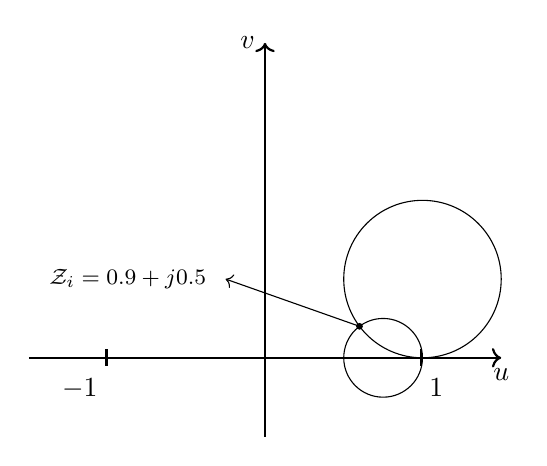
\begin{tikzpicture}
            % Axis
            \draw [thick,-|,black] (-3,0) -- (-2,0)
                node[label={below:$-1$},xshift=-1em] {};
                \draw [thick,-|,black] (-2,0) -- (2,0)
                node[label={below:$1$},xshift=0.5em] {};
            \draw[thick,->,black] (2,0)--(3,0) node[below] {$u$}; % x axis
            \draw[thick,->,black] (0,-1)--(0,4) node[left] {$v$}; % y axis
            \draw[->,black] (1.2,0.4)--(-0.5,1)
            node[label={[font=\footnotesize]left:$\mathcal{Z}_i = 0.9 +j0.5$}] {};
            \filldraw [black] (1.2,0.4) circle (1pt);
            \draw[black] (2*1,2*1/2) circle (2*1/2);
            \draw[black] (3*2/4,0) circle (2/4);
           \end{tikzpicture}
    \end{center}\caption{Smith Chart of $\mathcal{Z}_i = 2+j3$}\label{fig:example2_plot} 
\end{figure}
Then what we can do is to look at the reflection coefficient $\rho$, not only by looking ad $u$ and $v$, but obtaining the module and the phase of the complex vector $\rho$. You can see the example in \cref{fig:example2_rho}
\begin{figure}[H]
    \begin{center}
        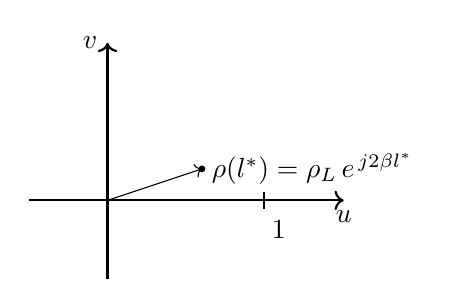
\begin{tikzpicture}
            % Axis
                \draw [thick,-|,black] (-1,0) -- (2,0)
                node[label={below:$1$},xshift=0.5em] {};
            \draw[thick,->,black] (2,0)--(3,0) node[below] {$u$}; % x axis
            \draw[thick,->,black] (0,-1)--(0,2) node[left] {$v$}; % y axis
            \filldraw [black] (1.2,0.4) circle (1pt);
            \draw[->,black] (0,0)--(1.2,0.4)node[right] {$\rho(l^*)=\rho_L\,e^{\,j2\beta l^*}$};;
           \end{tikzpicture}
    \end{center}\caption{Smith Chart of $\mathcal{Z}_i = 2+j3$}\label{fig:example2_rho} 
\end{figure}
According to \cref{eq:reflection_coeff_at_load2}, the module of the $\rho$ vector that we have found in the Smith chart is $\rho_L$ and it's phase angle is $2\beta l$.\\
This phase angle is very important, this is why you can find it already printed in the first outer diameter of the Smith chart, usually under the name of \emph{angle of reflection coefficient in degrees}.\\
If we move in the transmission line changing the $l$ value, in the Smith chart we will see that we are rotating the $\rho$ complex vector, but we don't change its module, like in \cref{fig:example2_rho2} 
\begin{figure}[H]
    \begin{center}
        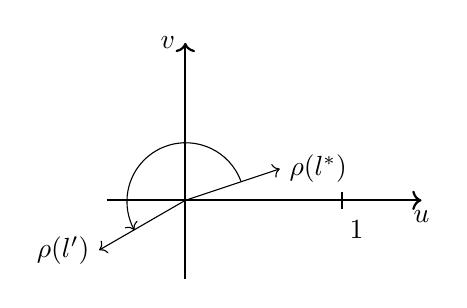
\begin{tikzpicture}
            % Axis
                \draw [thick,-|,black] (-1,0) -- (2,0)
                node[label={below:$1$},xshift=0.5em] {};
            \draw[thick,->,black] (2,0)--(3,0) node[below] {$u$}; % x axis
            \draw[thick,->,black] (0,-1)--(0,2) node[left] {$v$}; % y axis
            \draw[->,black] (0,0)--(1.2,0.4)node[right] {$\rho(l^*)$};
            \draw[black,thin, ->] (0.7071,0.24) arc (20:209:0.74672);
            \draw[->,black] (0,0)--(-1.09541,-0.6324555)node[left] {$\rho(l^\prime$)};
           \end{tikzpicture}
    \end{center}\caption{Smith Chart when we move on the line}\label{fig:example2_rho2} 
\end{figure}
We can exploit this cool behavior of the chart because whenever we move along the line, $\rho$ will rotate, and then we move in another point where we can interpolate the famous circles and we can obtain the value of the new $Z_i$ without going troughs all the ugly formulas that we have already seen before.\\
Another interesting characteristic of this chart is that when you rotate the vector, and touch the horizontal $u$ axe, the impedance will be completely real.

If from my point i do a complete rotation, this mean that my phase variation is $2\pi$, this mean that:
\begin{align}
    \begin{split}
        &2\beta l=2\pi\\[5pt]
        2 \frac{\cancel{2\pi}}{\lambda}l&=\cancel{2\pi}\\[5pt]
    \end{split}\label{eq:phase_rotation_smith}
\end{align}
We can see in \cref{eq:phase_rotation_smith} that by completing a rotation we are moving over the line by $l=\frac{\lambda}{2}$. This is true for every rotation, so in the outer diameters of the Smith chart .\\
It is interesting to see that if we move by $l=\frac{\lambda}{4}$ we are rotating by $180\si{\degree}$, and if we look at the impedance we notice that $\mathcal{Z}_a=\frac{1}{\mathcal{Z}_b}$ as expected.\\
In the outer diameter of the Smith chart we can see also that is marked the how far we are moving from or towards the load normalized by the $\lambda$. We know also the direction because if we are moving towards the load mean that the $l$ value is increasing, and thus the angle of $\rho$, so we are moving anticlockwise in the chart.

%%--- VERY BIG SMITH CHART, TO CONTINUE TEXT SCROLL UNTIL LINE 690 ---%
\begin{figure}[H]
    \begin{center}
        \resizebox{1\textwidth}{!}{
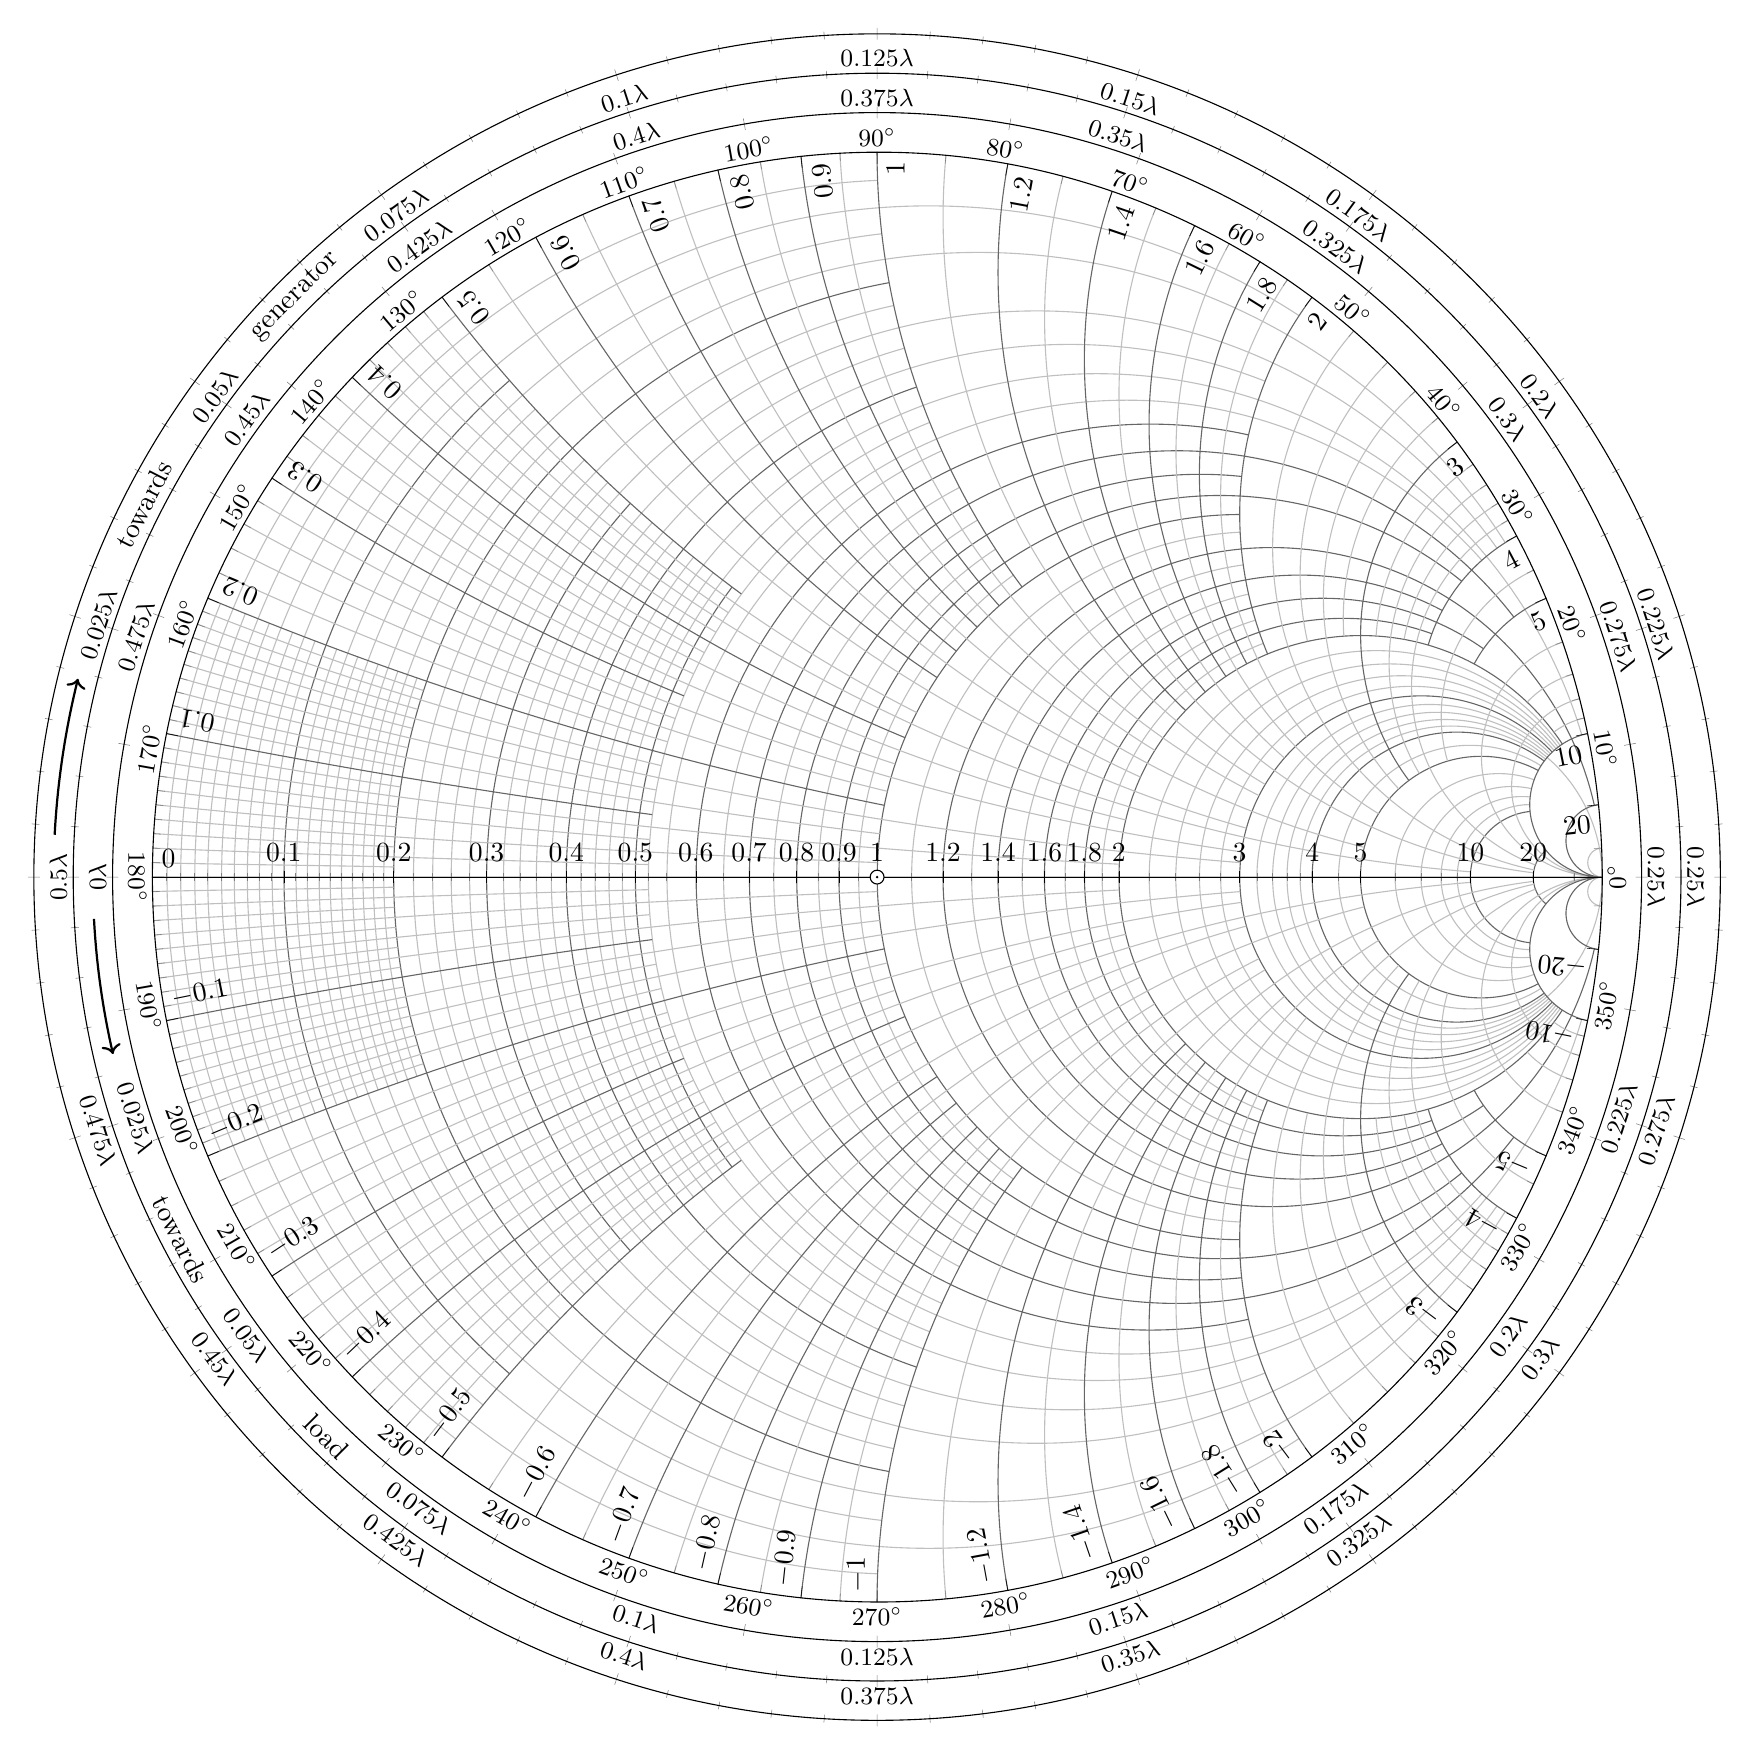
\begin{tikzpicture}
    \pgfmathsetmacro{\xoffset}{10.45*(1-cos(3))-1.25}  
    \pgfmathsetmacro{\yoffset}{sin(3)*10.45+9.2}  
    \draw[,thick,->] (+\xoffset,\yoffset) arc [radius=10.45cm,start angle=177,end angle=166];
    \pgfmathsetmacro{\xoffset}{10.45*(1-cos(18))-1.25}  
    \pgfmathsetmacro{\yoffset}{sin(18)*10.45+9.2} 
    \draw[,draw=none] (+\xoffset,\yoffset) arc [radius=10.45cm,start angle=162,end angle=144] node[midway,sloped]{towards};
    \pgfmathsetmacro{\xoffset}{10.45*(1-cos(36))-1.25}  
    \pgfmathsetmacro{\yoffset}{sin(36)*10.45+9.2} 
    \draw[,draw=none] (+\xoffset,\yoffset) arc [radius=10.45cm,start angle=144,end angle=126] node[midway,sloped]{generator};

    \pgfmathsetmacro{\xoffset}{9.95*(1-cos(-3))-0.75}  
    \pgfmathsetmacro{\yoffset}{sin(-3)*9.95+9.2} 
    \draw[,thick,->] (\xoffset,\yoffset) arc [radius=9.95cm,start angle=183,end angle=193] ;
    \pgfmathsetmacro{\xoffset}{9.95*(1-cos(-18))-0.75}  
    \pgfmathsetmacro{\yoffset}{sin(-18)*9.95+9.2} 
    \draw[,draw=none] (+\xoffset,\yoffset) arc [radius=10.45cm,start angle=198,end angle=216] node[midway,sloped]{towards};
    \pgfmathsetmacro{\xoffset}{9.95*(1-cos(-36))-0.75}  
    \pgfmathsetmacro{\yoffset}{sin(-36)*9.95+9.2} 
    \draw[,draw=none] (+\xoffset,\yoffset) arc [radius=10.45cm,start angle=216,end angle=234] node[midway,sloped]{load};


  \begin{polaraxis}[
                    rotate=180,
                    width=23cm,
                    xshift=1.5cm, 
                    yshift=1.5cm,
                    %xticklabels={$0\lambda$,$0.05\lambda$,$0.1\lambda$,$0.15\lambda$,$0.2\lambda$,$0.25\lambda$},
                    xticklabel style={
                        sloped like x axis={%
                            execute for upside down={\tikzset{anchor=south}},
                            reset nontranslations=false
                        },
                        anchor=north,
                    },
                    xticklabel={\small\pgfmathparse{0.5-\tick/720}\pgfmathprintnumber[fixed,precision=3]{\pgfmathresult}$\lambda$},
                    xtick align=center,
                    xtick={0,18,...,360},
                    grid=none,
                    axis y line = none,
                    minor x tick num={4},
                    ymax=1,
                   ]   
 \end{polaraxis}

  \begin{polaraxis}[
                    rotate=180,
                    width=22cm,
                    xshift=1cm, 
                    yshift=1cm,
                    %xticklabels={$0\lambda$,$0.05\lambda$,$0.1\lambda$,$0.15\lambda$,$0.2\lambda$,$0.25\lambda$},
                    xticklabel style={
                        sloped like x axis={%
                            execute for upside down={\tikzset{anchor=south}},
                            reset nontranslations=false
                        },
                        anchor=north,
                    },
                    xticklabel={\small\pgfmathparse{\tick/720}\pgfmathprintnumber[fixed,precision=3]{\pgfmathresult}$\lambda$},
                    xtick align=center,
                    xtick={0,18,...,360},
                    grid=none,
                    axis y line = none,
                    minor x tick num={4},
                    ymax=1,
                   ]    

  \end{polaraxis}



  \begin{polaraxis}[
                    width=21cm,
                    xshift=-0.5cm, 
                    yshift=-0.5cm,
                    %xticklabels={$0\lambda$,$0.05\lambda$,$0.1\lambda$,$0.15\lambda$,$0.2\lambda$,$0.25\lambda$},
                    xticklabel style={
                        sloped like x axis={%
                            execute for upside down={\tikzset{anchor=north}},
                            reset nontranslations=false
                        },
                        anchor=south,
                    },
                    xticklabel={\small\pgfmathprintnumber{\tick}\si{\degree}},
                    xtick align=center,
                    grid=none,
                    axis y line = none,
                   ]    
 \end{polaraxis}

 \begin{smithchart}[
                    show origin,
                    width=20cm,
                   ]
 \end{smithchart}
 \end{tikzpicture}
    }
\end{center}\caption{Smith chart}\label{fig:beautiful_smith}
\end{figure}
%%--- very big smith chart finished ---%%



%\begin{figure}[H]
%    \begin{center}
%        \begin{tikzpicture}
%            \begin{smithchart}[
%            title=Smith Chart Stub Matching,
%            width=1\textwidth,
%            ]
%            \end{smithchart}
%        \end{tikzpicture}
%    \end{center}
%\end{figure}

\medskip
\bibliographystyle{unsrt}
\bibliography{bibliography}

\end{document}
